\chapter{Selection and Categorisation}
\label{chap:selection_and_categorisation}
\chapterquote{Science never solves a problem without creating ten more.}
{George Bernard Shaw, 1856 -- 1950}

This thesis presents results of three different analyses used in the Higgs to two photon search at CMS. The nominal results and properties are obtained from the so called \MFM analysis, which uses multivariate methods optimised specifically to search for a \SM Higgs boson to select and categorise events. Two further analyses are presented as cross checks to the baseline \MFM analysis. The first, the \CiC analysis, is designed for simplicity and robustness as a cut based approach and, owing to its low level of model dependence, is used for the spin analysis. The second, the \SMVA analysis, serves to cross check the background, the most significant unknown in a search like this, and categorisation by extracting the background under the signal region from sidebands in the diphoton invariant mass spectrum.

Both the \CiC and \MFM analyses have a fully parametric definition of the diphoton invariant mass spectrum where the signal shape is derived from \MC simulation. The \SMVA uses a cut and count method. 


% ---- SECTION ----
\section{Event selection}
\label{sec:event_selection}

There are two complimentary event selections used in the three analyses. The \CiC analysis uses a cut based photon selection whilst the \MFM and \SMVA analyses use a series of \BDTs to first select photons and then select events. The ultimate aim is a selection which accepts two prompt photons (i.e.\ does not contain any fakes) and exploits regions of phase space which have a narrow mass resolution and high signal to background ratio.

All events must contain at least two photons which pass $p_{T}^{\gamma_{1}}>m_{\gamma\gamma}/3$ (for the leading photon) and $p_{T}^{\gamma_{2}}>m_{\gamma\gamma}/4$ (for the subleading photon) and the invariant mass of the diphoton pair must be in the range $100<m_{\gamma\gamma}<180$. In the case where there are more than two photon candidates in an event, the two photons which give the highest scalar sum \pT are chosen. 

\subsection{Selection using cuts in categories}
\label{sec:cic}

Cuts are optimised for photons in four non-overlapping categories to take advantage of the different photon energy resolution between the barrel and the endcap and between converted and non-converted photons. The categories are defined as $|\eta|<1.444$ or $|\eta|>1.556$ (i.e.\ either barrel or endcap) and $R_{9}<0.94$ or $R_{9}\geq 0.94$ (i.e.\ either converted or non-converted) and the cuts are chosen by targeting a specific signal to background ratio ($S/B$). The procedure to define the cuts is as follows,

\begin{itemize}
  \item A set of loose cuts are defined as the starting values.
  \item The ``N-1" distribution of each cut variable is produced. This is the distribution of each variable after the cuts on all other variables have been applied.
  \item A smooth curve is fitted to the distribution of the $B/S$ ratio versus the cut variable.
  \item The cut value is chosen by evaluating the curve for the required value of $S/B$.
  \item Do the same for all the other variables.
\end{itemize}

Consequently a stable set of cut values is obtained by iterating this procedure a few times. Each cut will then select events with the same purity ($S/B$) and thus the efficiency for selected photons is maximised for the chosen purity level. As a result the cuts in the endcap are much tighter than in the barrel, similarly the cuts for low \rnine photons are much tighter than the cuts for high \rnine photons. The cut variables are described below and the cut values shown in Table~\ref{tab:cic_cuts}. The cut setting procedure is optimised on a signal sample of \Hgg MC (with \mH=120\GeV) and a background sample of \gjet events. The photon efficiency of the cuts for the four different classes of photon is shown in Figure~\ref{fig:cic_efficiency} as a function of the supercluster position, \eta, and the photon \pT.

\begin{itemize}
  \item \textbf{PF isolation sum, chosen vertex} - Sum of particle flow photon, charged and neutral hadron isolation sums defined in Sec.~\ref{sec:iso} where all \PF candidates originate from the primary vertex selected in Sec.~\ref{sec:vtx_reco}
  \item \textbf{PF isolation sum, worst vertex} - As above but where all \PF candidates originate instead from the vertex which gives the largest charged hadron PF isolation sum. This add protection for cases when the primary vertex is incorrectly assigned.
  \item \textbf{Charged PF isolation sum} - Described above in Sec.~\ref{sec:iso}
  \item \boldmath{$\sigma_{i\eta i\eta}$} - Described above in Sec.~\ref{sec:photon_presel}
  \item \boldmath{$H/E$} - Described above in Sec.~\ref{sec:photon_presel}
  \item \boldmath{$R_{9}$} - Described above in Sec.~\ref{sec:ecal}
\end{itemize}

\begin{table}
  \begin{center}
    \begin{tabular}{l l l l l}
      & \multicolumn{2}{c}{Barrel} & \multicolumn{2}{c}{Endcap} \\ 
      & \multicolumn{1}{l}{\rnine $>$ 0.94} & \multicolumn{1}{l}{\rnine $<$ 0.94 } & \multicolumn{1}{l}{\rnine $>$ 0.94 } & \multicolumn{1}{l}{\rnine $<$ 0.94 } \\ 
      \hline
      PF isolation sum, chosen vertex & $<$6 & $<$4.7 & $<$5.6 & $<$3.6 \\ 
      PF isolation sum, worst vertex & $<$10 & $<$6.5 & $<$5.6 & $<$4.4 \\ 
      Charged PF isolation sum & $<$3.8 & $<$2.5 & $<$3.1 & $<$2.2 \\ 
      $\sigma_{i\eta i\eta}$ & $<$0.0108 & $<$0.0102 & $<$0.028 & $<$0.028 \\ 
      H/E & $<$0.124 & $<$0.092 & $<$0.142 & $<$0.063 \\ 
      \rnine & $>$0.94 & $>$0.298 & $>$0.94 & $>$0.24 \\ 
    \end{tabular}
  \end{center}
  \caption{Photon ID selection cut values. The cuts are applied to both the leading and subleading photons.}
  \label{tab:cic_cuts}
\end{table}

\begin{figure}
  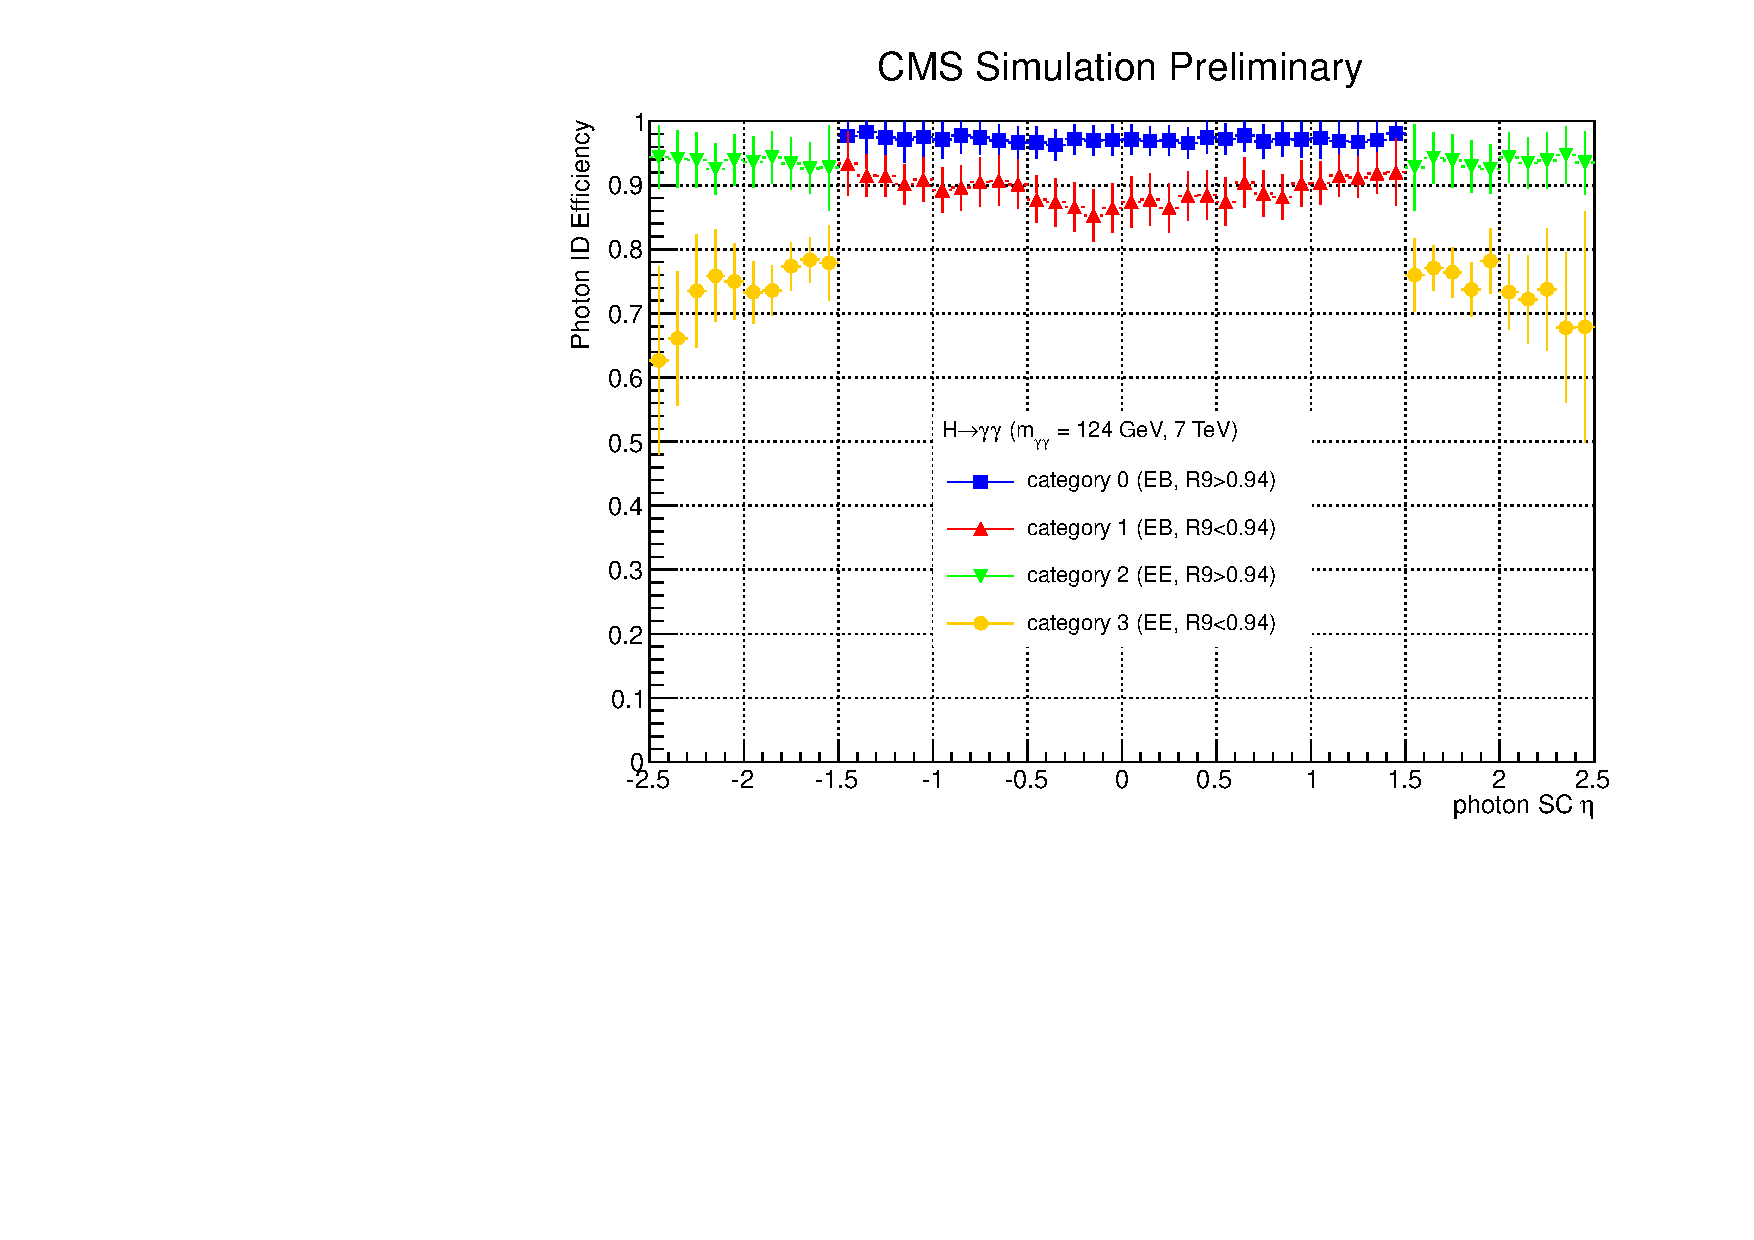
\includegraphics[width=0.48\textwidth]{selec_and_cats/plots/eff_7TeV_eta.pdf}
  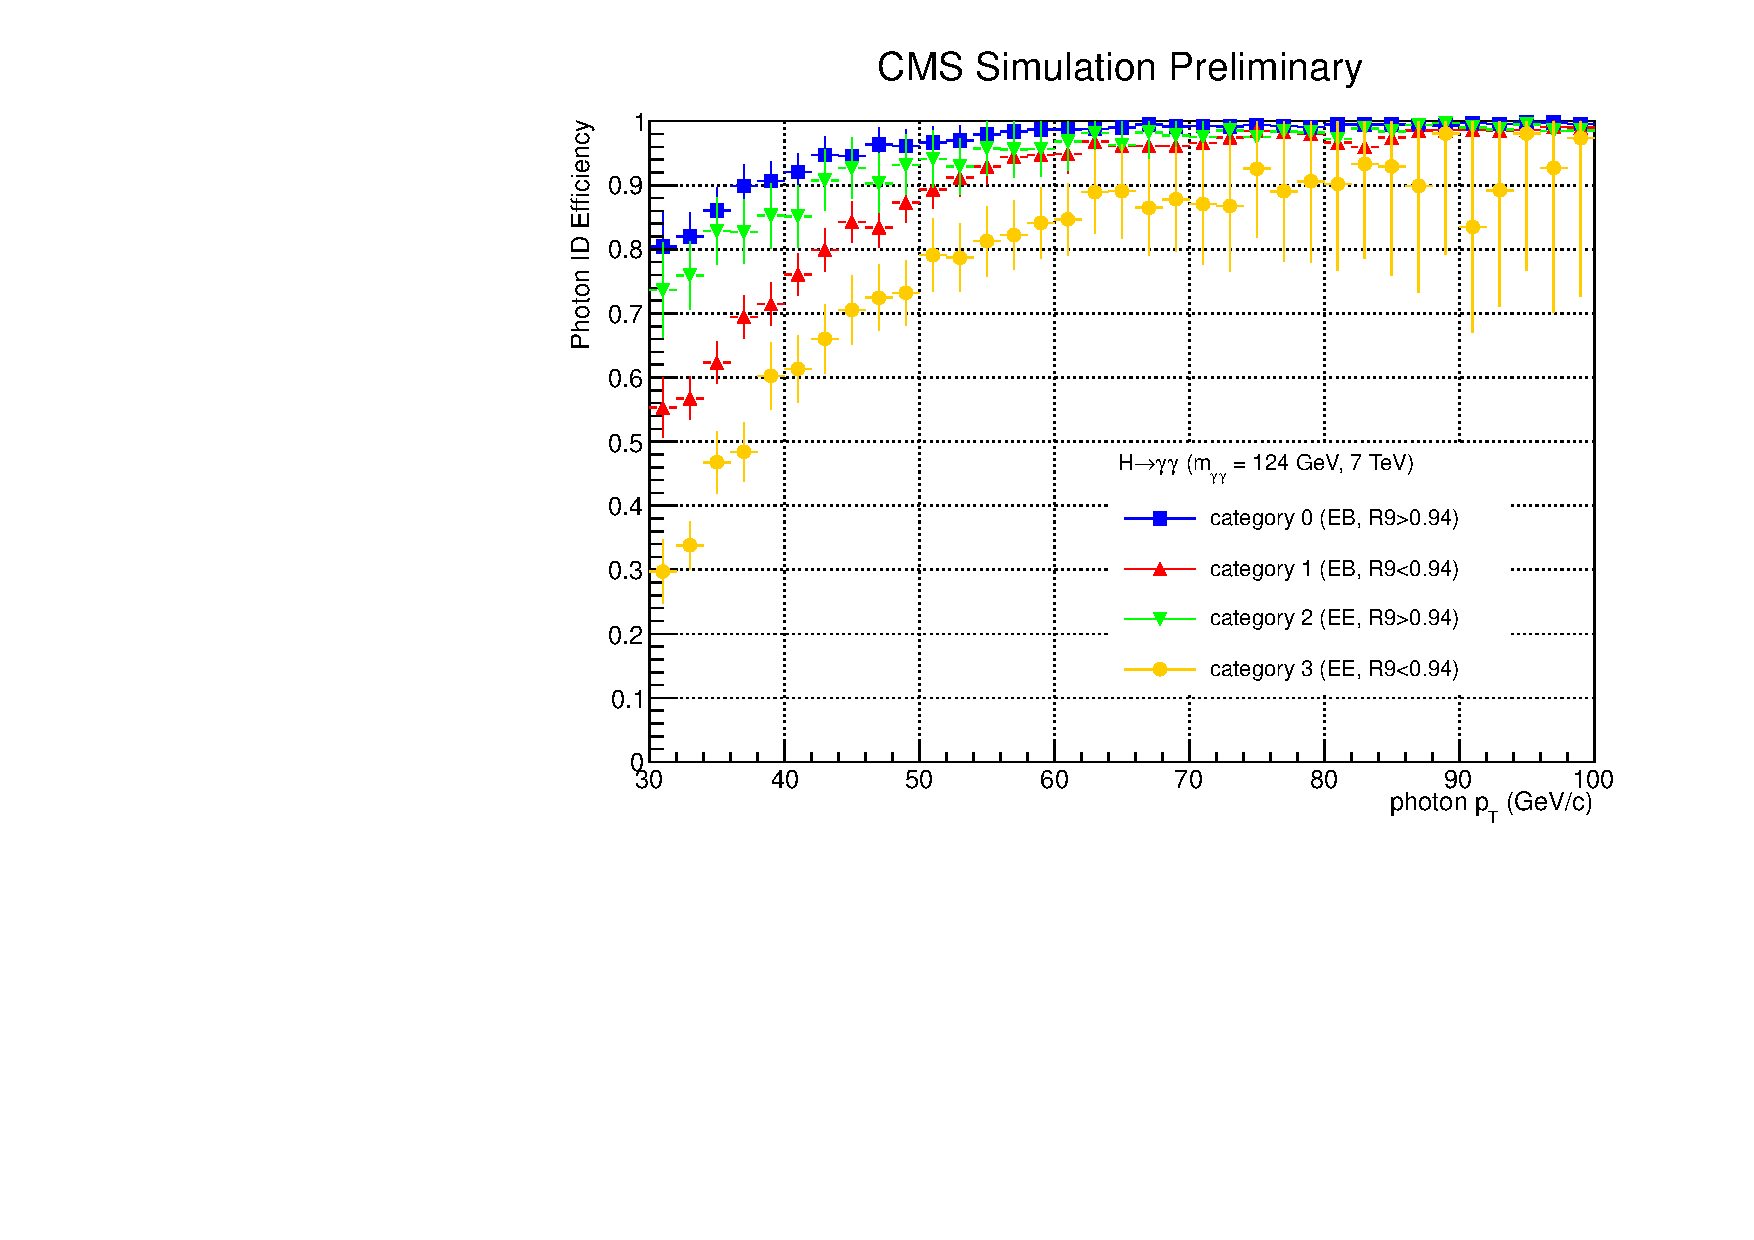
\includegraphics[width=0.48\textwidth]{selec_and_cats/plots/eff_7TeV_pt.pdf}
  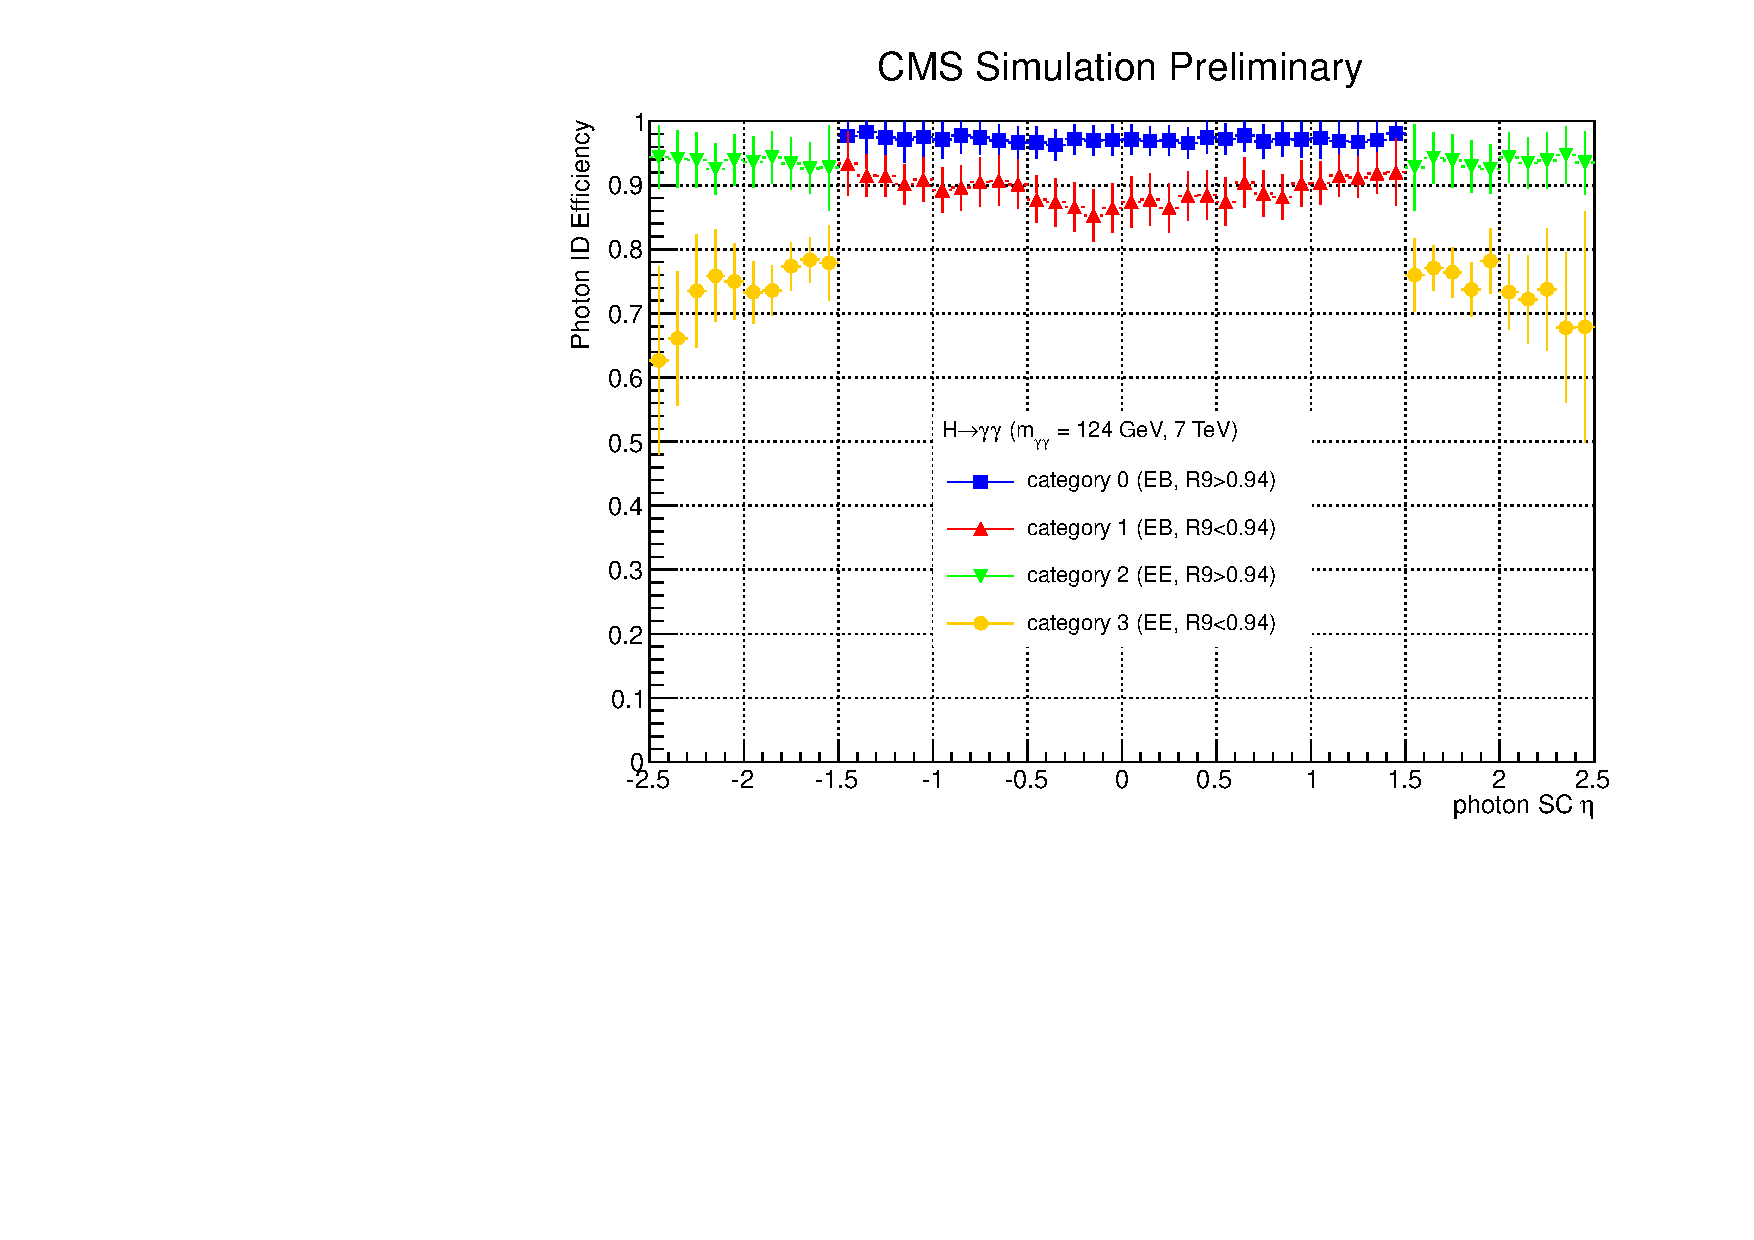
\includegraphics[width=0.48\textwidth]{selec_and_cats/plots/eff_7TeV_eta.pdf}
  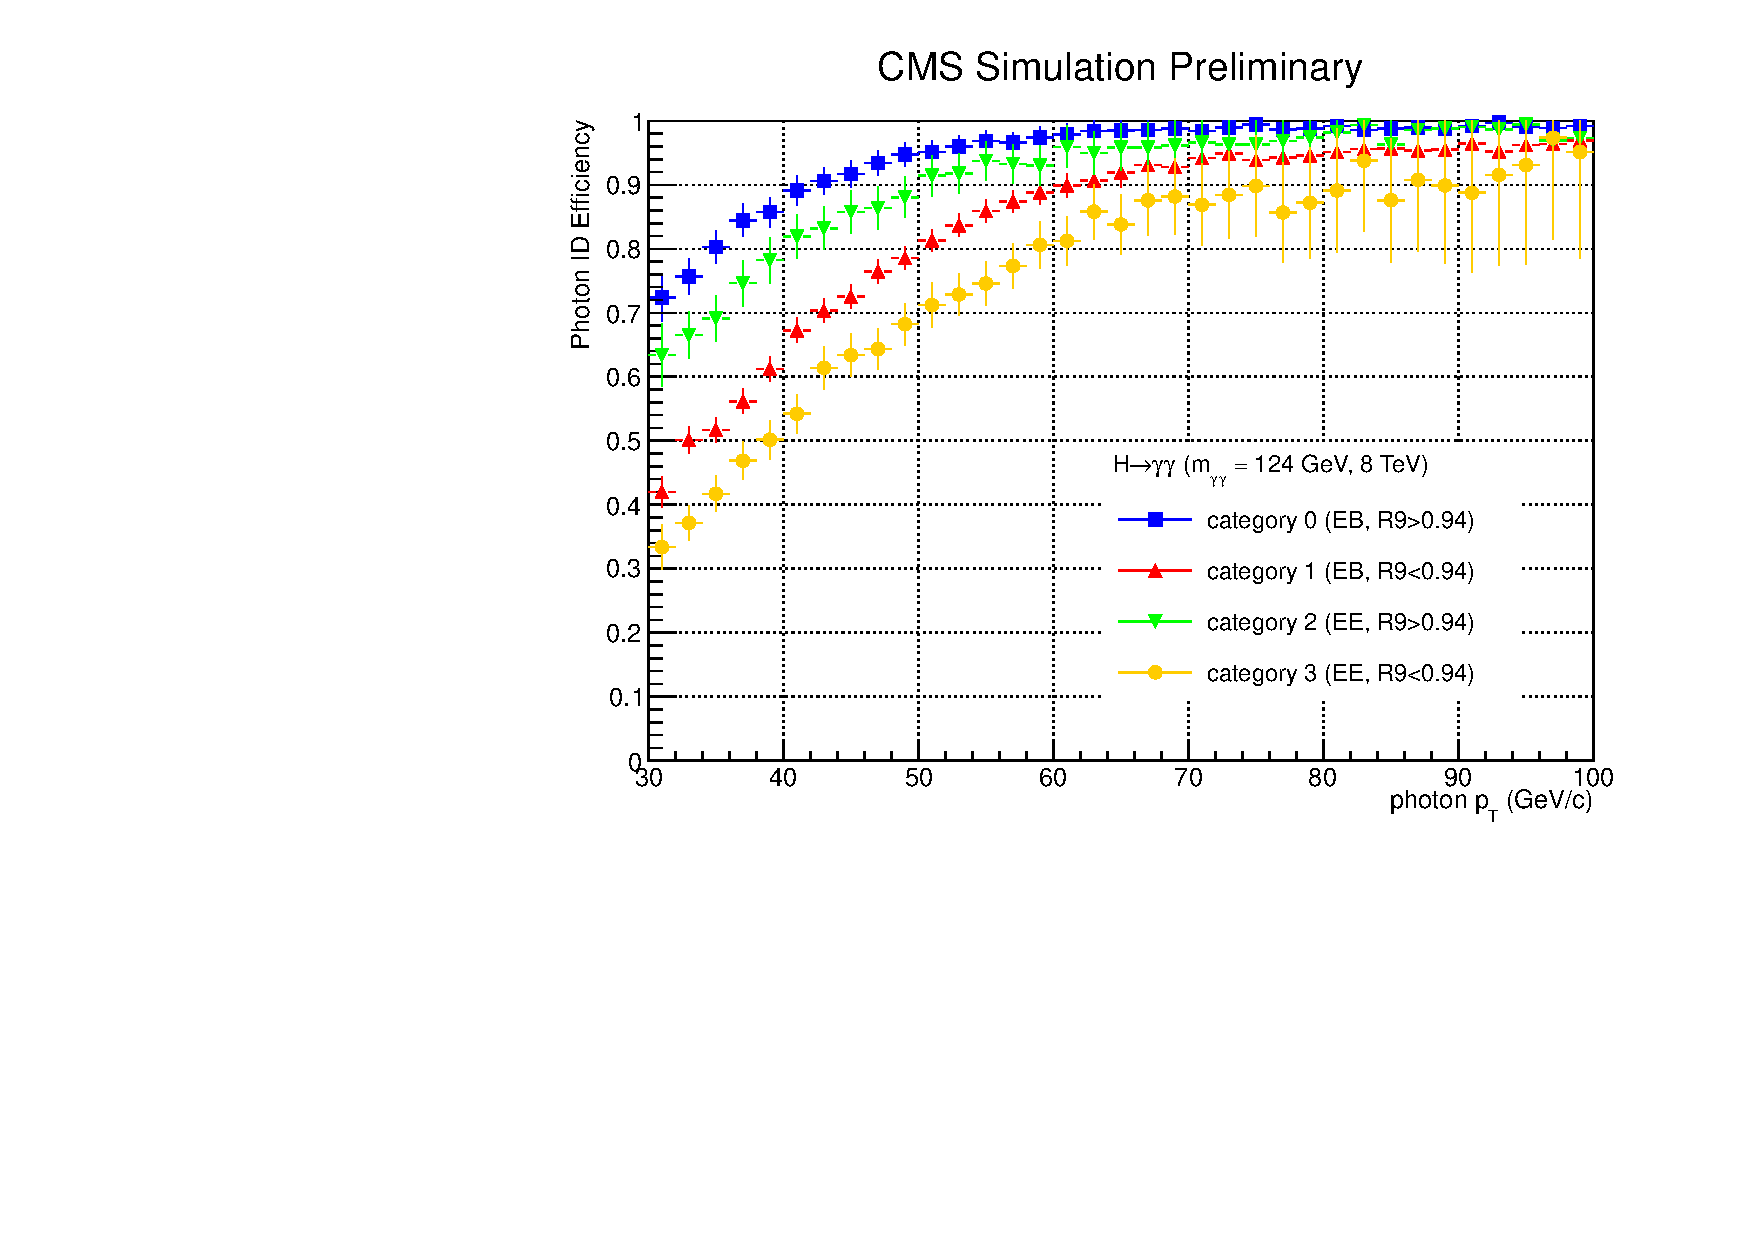
\includegraphics[width=0.48\textwidth]{selec_and_cats/plots/eff_8TeV_pt.pdf}
  \caption{Cut based photon ID efficiency as measured in \Zee tag and probe. MORE DESCRIPTION}
  \label{fig:cic_efficiency}
\end{figure}

\subsection{Photon ID MVA}
\label{sec:pho_id_mva}

For the multivariate approach a \BDT is trained to discriminate between prompt photons and jets. The desire is to factorise the photon selection, which is required to distinguish prompt photons from neutral mesons faking photons, and the event selection, which is required to consider kinematics, resolution etc.~to distinguish \Hgg from the $pp\rightarrow\gamma\gamma, \gjet, \mathrm{jet}+\mathrm{jet}$ background. The input variables used are designed specifically to distinguish between photons and fakes and to decouple from any event or photon kinematics which make the identification Higgs specific. Consequently, the training samples used are \gjet samples where the identification \BDT signal is the prompt $\gamma$ and the background is the fake jet. The \pT and supercluster \eta distribution of the prompt photon are reweighted to match the background non-prompt photons in order to further negate any photon kinematics which the \BDT could exploit. The photon ID \BDT is trained separately for the barrel and endcap in both 7 and 8~\TeV as these regions of phase space are so different. The result is four separate trainings in total.

The input variables aim to exploit differences in the shower shape and isolation between prompt and non-prompt photons and the correlation between these variables and the supercluster position and energy. They are,

\noindent\textbf{Shower shape variables}
\begin{itemize}
  \item $\sigma_{i\eta i\eta}$ - Explained above in Sec.~\ref{sec:photon_presel}
  \item $\sigma^{2}_{i\eta i\phi}$ - The equivalent diagonal spread (in \eta,\phi) of the shower.
  \item $E_{2\times2}/E_{5\times5}$ - Ratio of energy in the most energetic 2$\times$2 cluster which contains the seed to the energy in the 5$\times$5 cluster.
  \item $R_{9}$ - Explained above in Sec.~\ref{sec:ecal}.
  \item $\sigma_{\eta}$ - The energy weighted standard deviation of single crystal eta within the supercluster.
  \item $\sigma_{\phi}$ - The energy weighted standard deviation of single crystal phi within the supercluster.
  \item $\sigma_{xy}$ (for endcap only) - The standard deviation of the shower spread in the $x$, $y$ planes of the preshower.
\end{itemize}

\noindent\textbf{Isolation variables}
\begin{itemize}
  \item PF Photon ISO - Particle flow photon isolation sum
  \item PF Charged Hadron ISO (selected vertex) - Particle flow charged hadron isolation sum for candidates originating from selected vertex.
  \item PF Charged Hadron ISO (worst vertex) - Particle flow charged hadron isolation sum for candidates originating from the vertex with the largest isolation sum.
\end{itemize}

\noindent\textbf{Correlation variables}
\begin{itemize}
  \item $\rho$ - The median energy density in the event.
  \item $\eta$ - The \eta position of the photon supercluster.
  \item $E_{raw}$ - The raw energy of the photon supercluster.
\end{itemize}

The testing sample used to verify the output of the photon identification \BDT is a \MC \Hgg sample (\mH=124\GeV). The photon identification \BDT output (which is shown for the four different trainings in Figure~\ref{fig:photon_id_bdt}) provides a measure of an individual photons' ``quality" and is used as an input to the event level \BDT (described in the next section). Even so, a considerable amount of background is cut out by defining a loose cut (the \BDT output must be $>-0.2$) on the photon ID \BDT output value which is more than 99\% signal efficient.

The photon ID \BDT response for each photon is used as a direct input to the event level \MVA. Given that imperfect modeling of the detector response can result in a small change in the photon ID response which has a direct impact on the event level \MVA response, which is used to classify events, a systematic on the photon quality is applied and propagated through to the event level \MVA. Validation of the photon ID \BDT response in the \Zee decay is shown in Figure~\ref{fig:photon_id_zee} with the size of the systematic shown. Validation is done with the \Zee decay on all of the input variables, these distributions are shown in Appendix~\ref{app:photon_id} (\red{this may not be entirely necessary})


\begin{figure}
  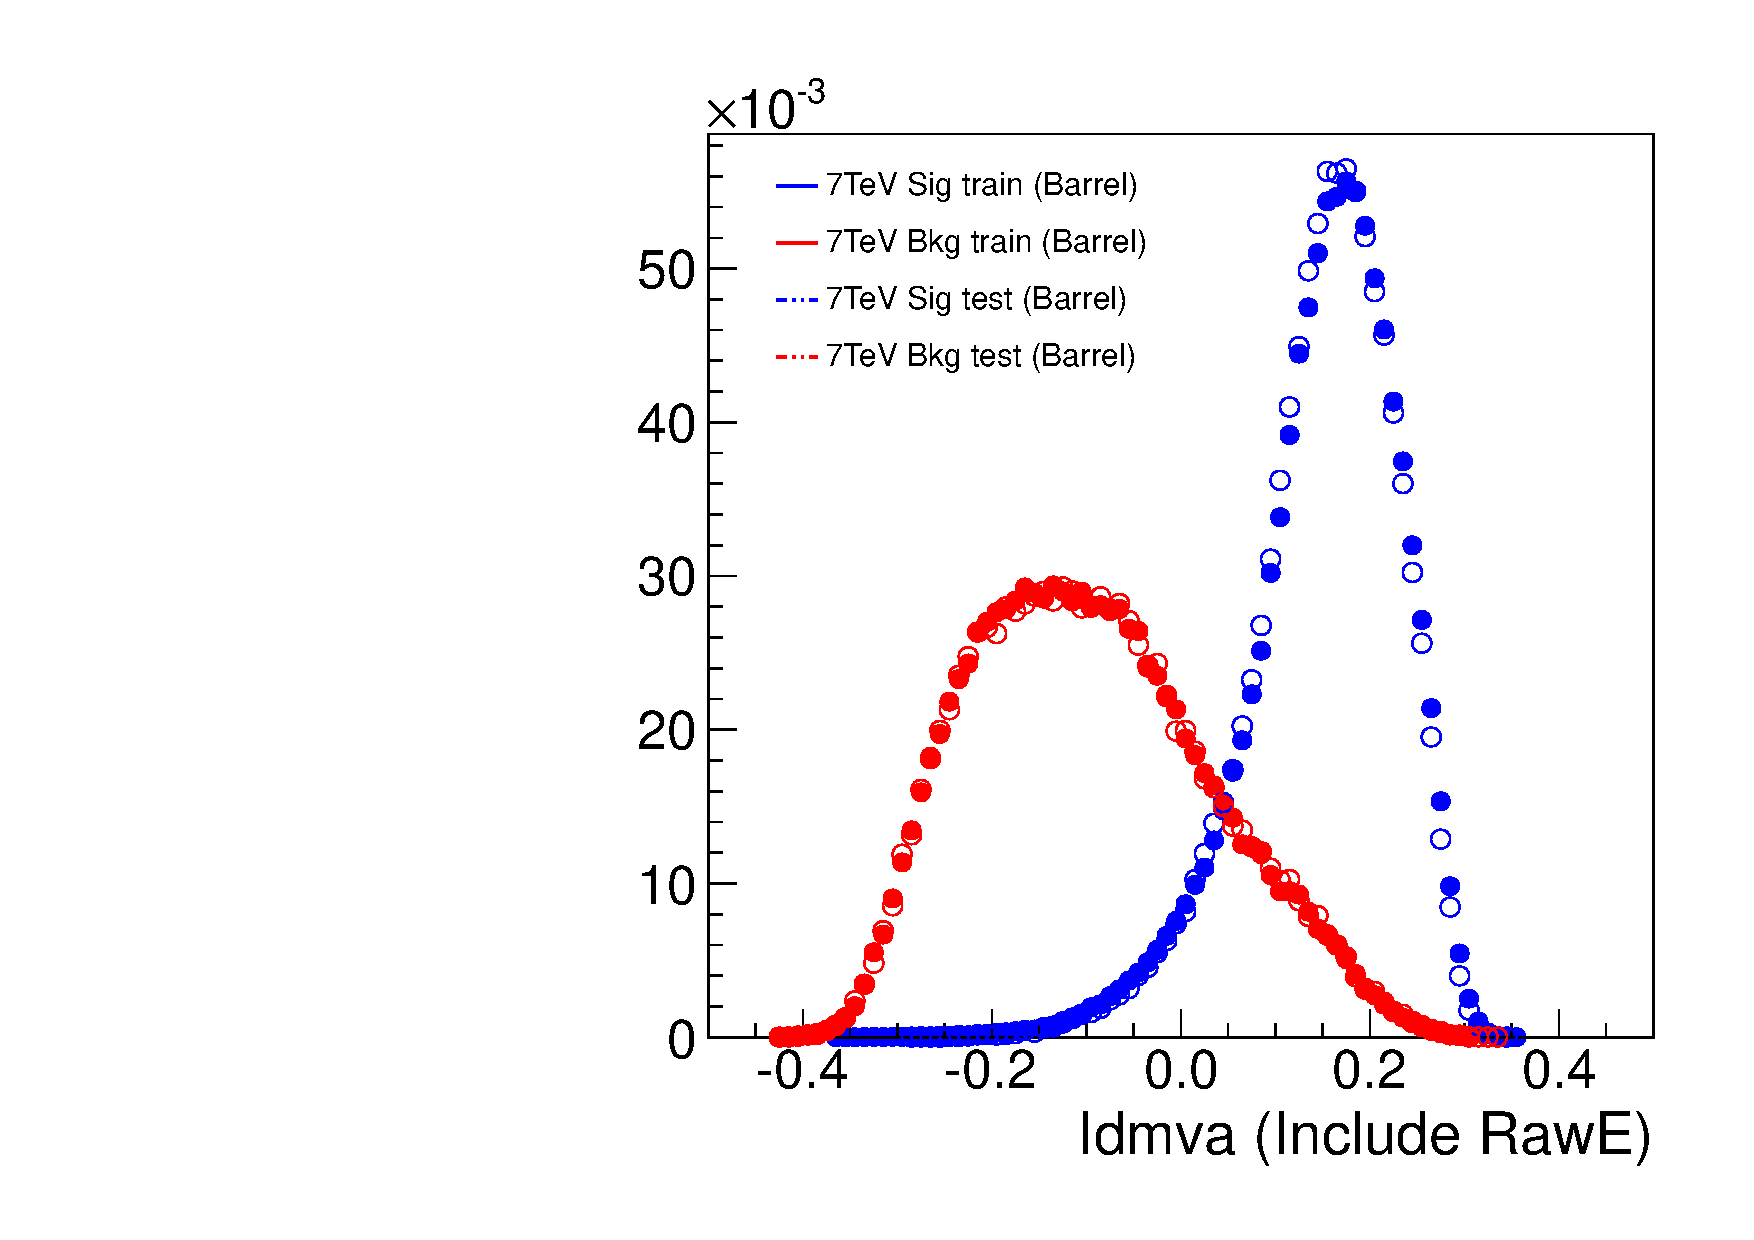
\includegraphics[width=0.48\textwidth]{selec_and_cats/plots/photonID_7TeV_barrel.pdf}
  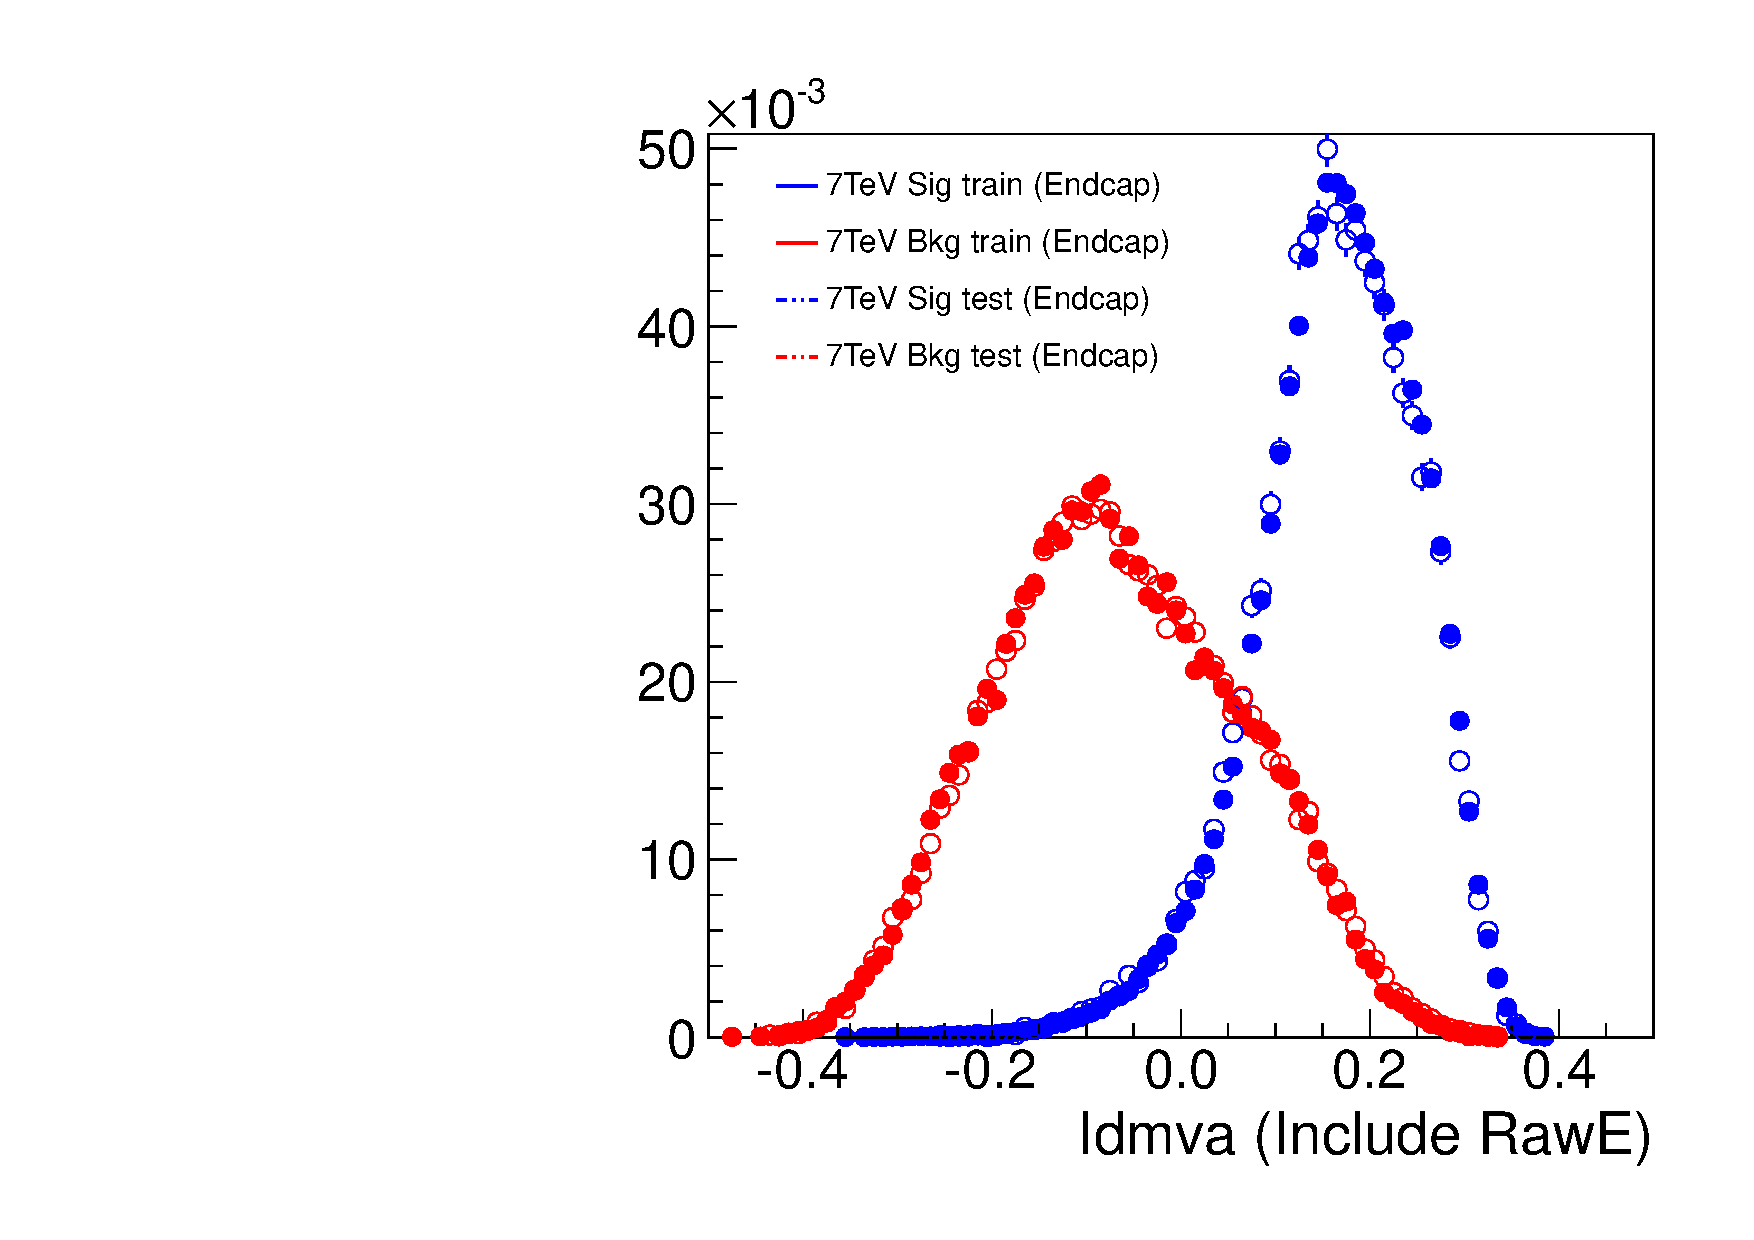
\includegraphics[width=0.48\textwidth]{selec_and_cats/plots/photonID_7TeV_endcap.pdf} \\
  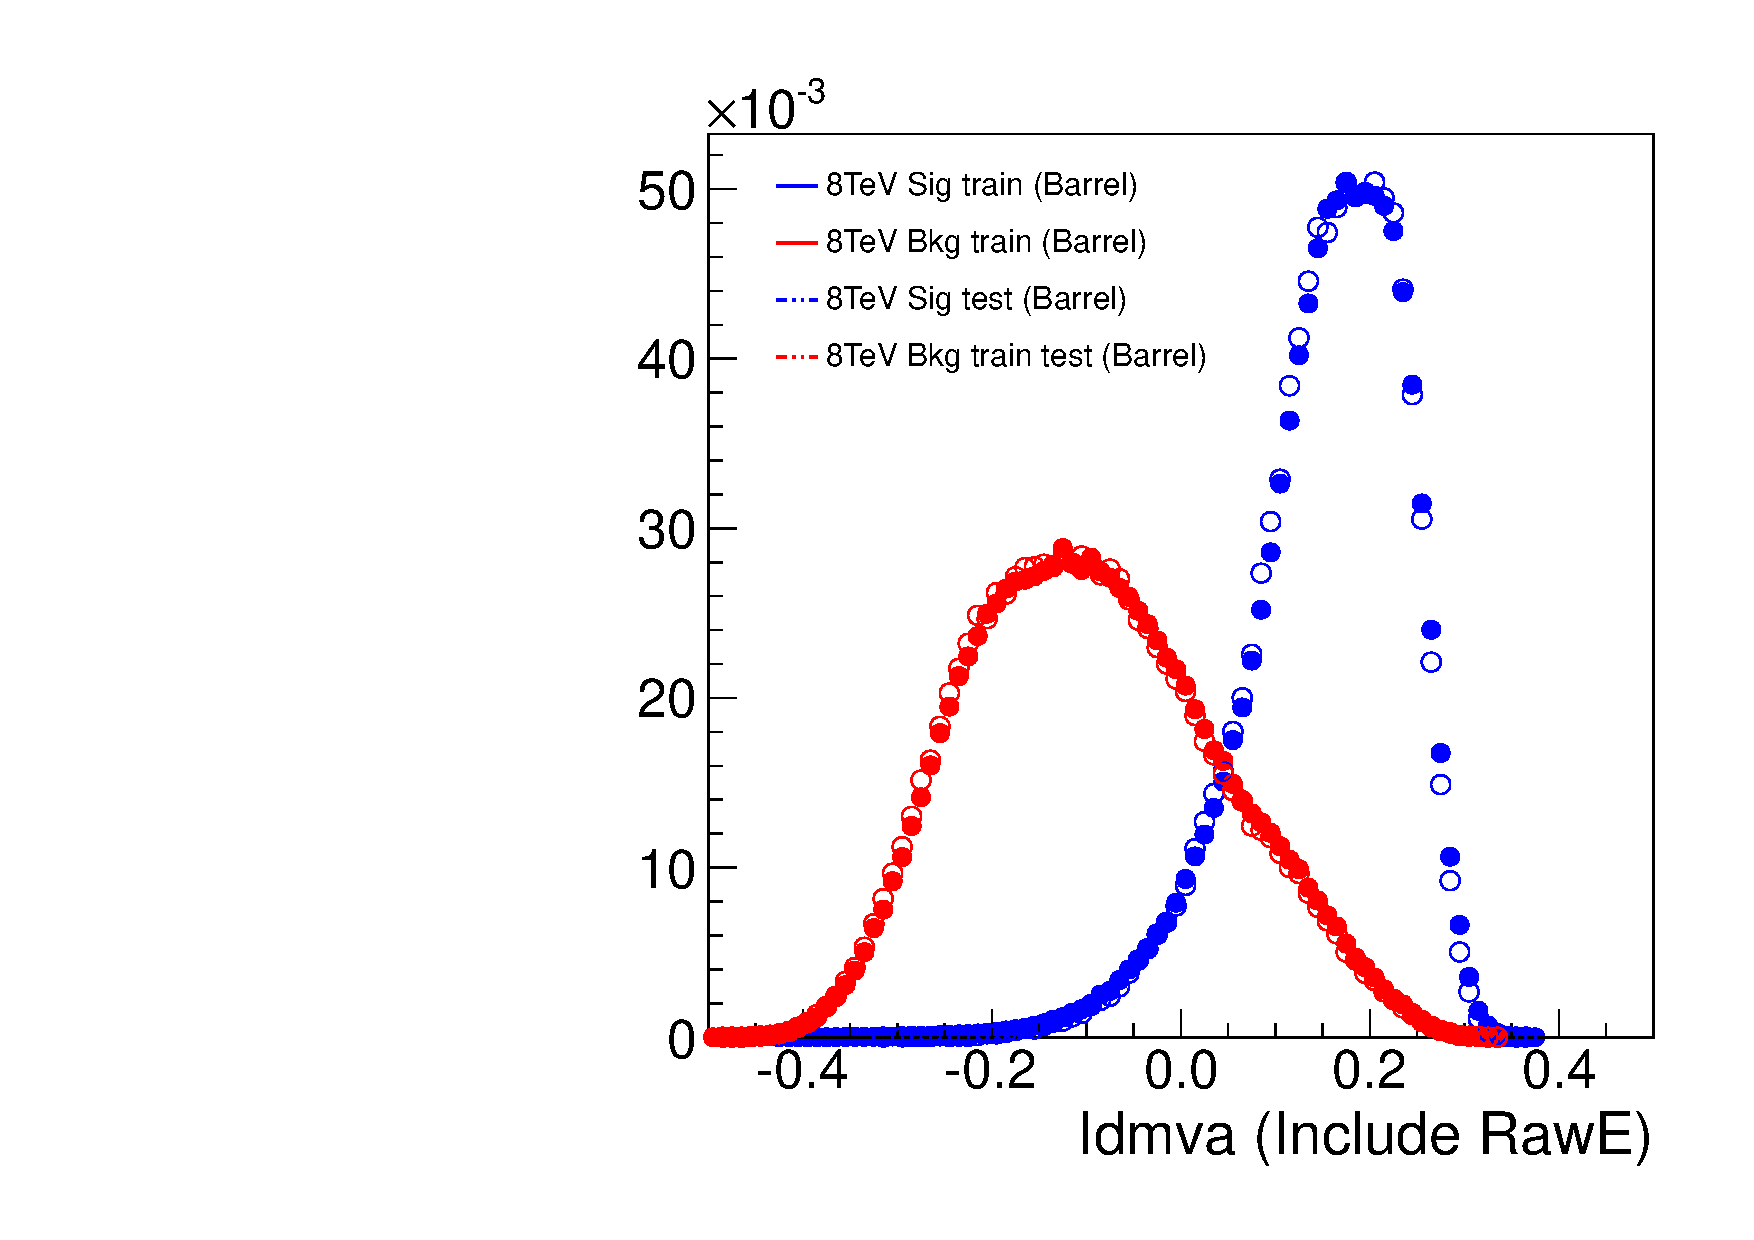
\includegraphics[width=0.48\textwidth]{selec_and_cats/plots/photonID_8TeV_barrel.pdf}
  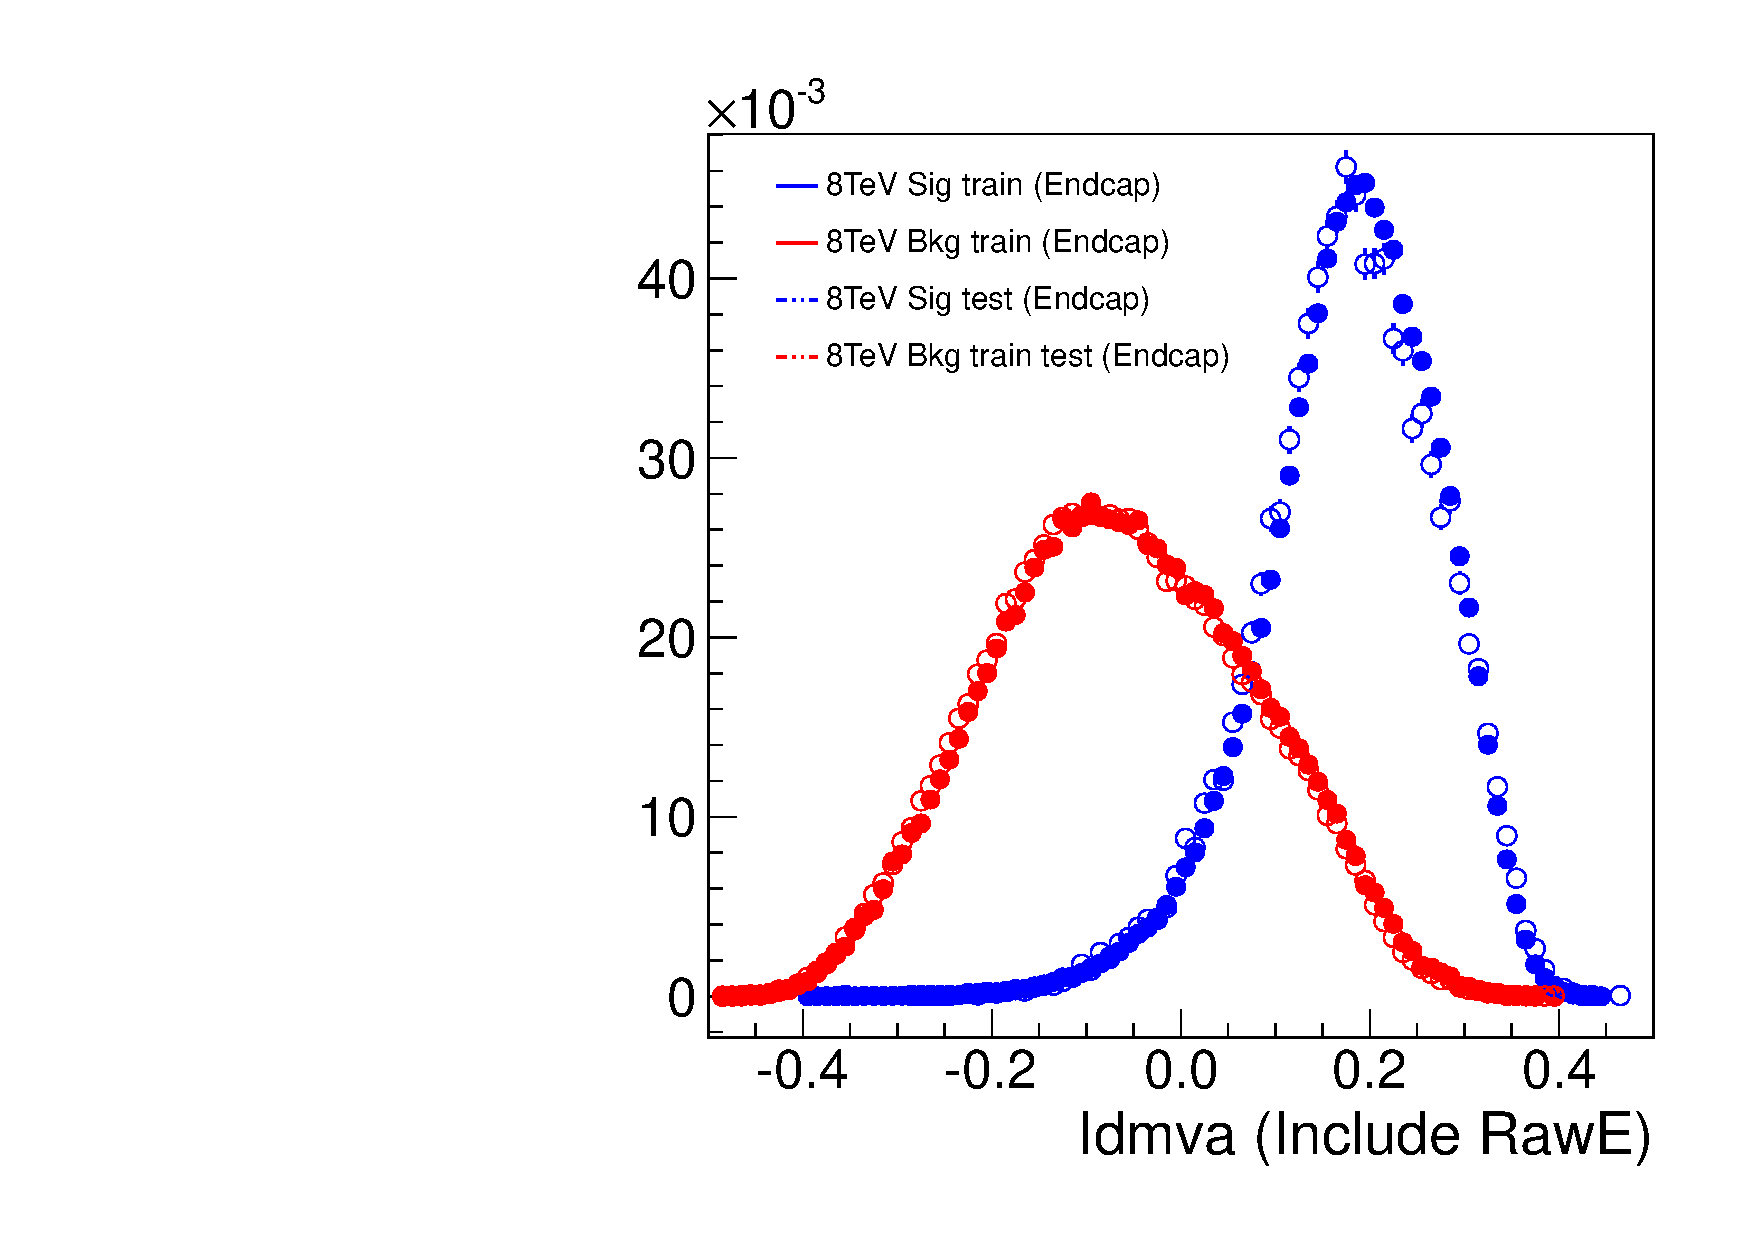
\includegraphics[width=0.48\textwidth]{selec_and_cats/plots/photonID_8TeV_endcap.pdf}
  \caption{The output distribution of the photon identification \BDT for 7\TeV barrel (top left), 7\TeV endcap (top right), 8\TeV barrel (bottom left) and 8\TeV endcap (bottom right). The solid points show the \gjet training sample distributions and the hollow points show the \Hgg test sample distributions for prompt signal photons in blue and fake background photons in red. A cut of $>-0.2$ is made on all photons.}
  \label{fig:photon_id_bdt}
\end{figure}

\begin{figure}
  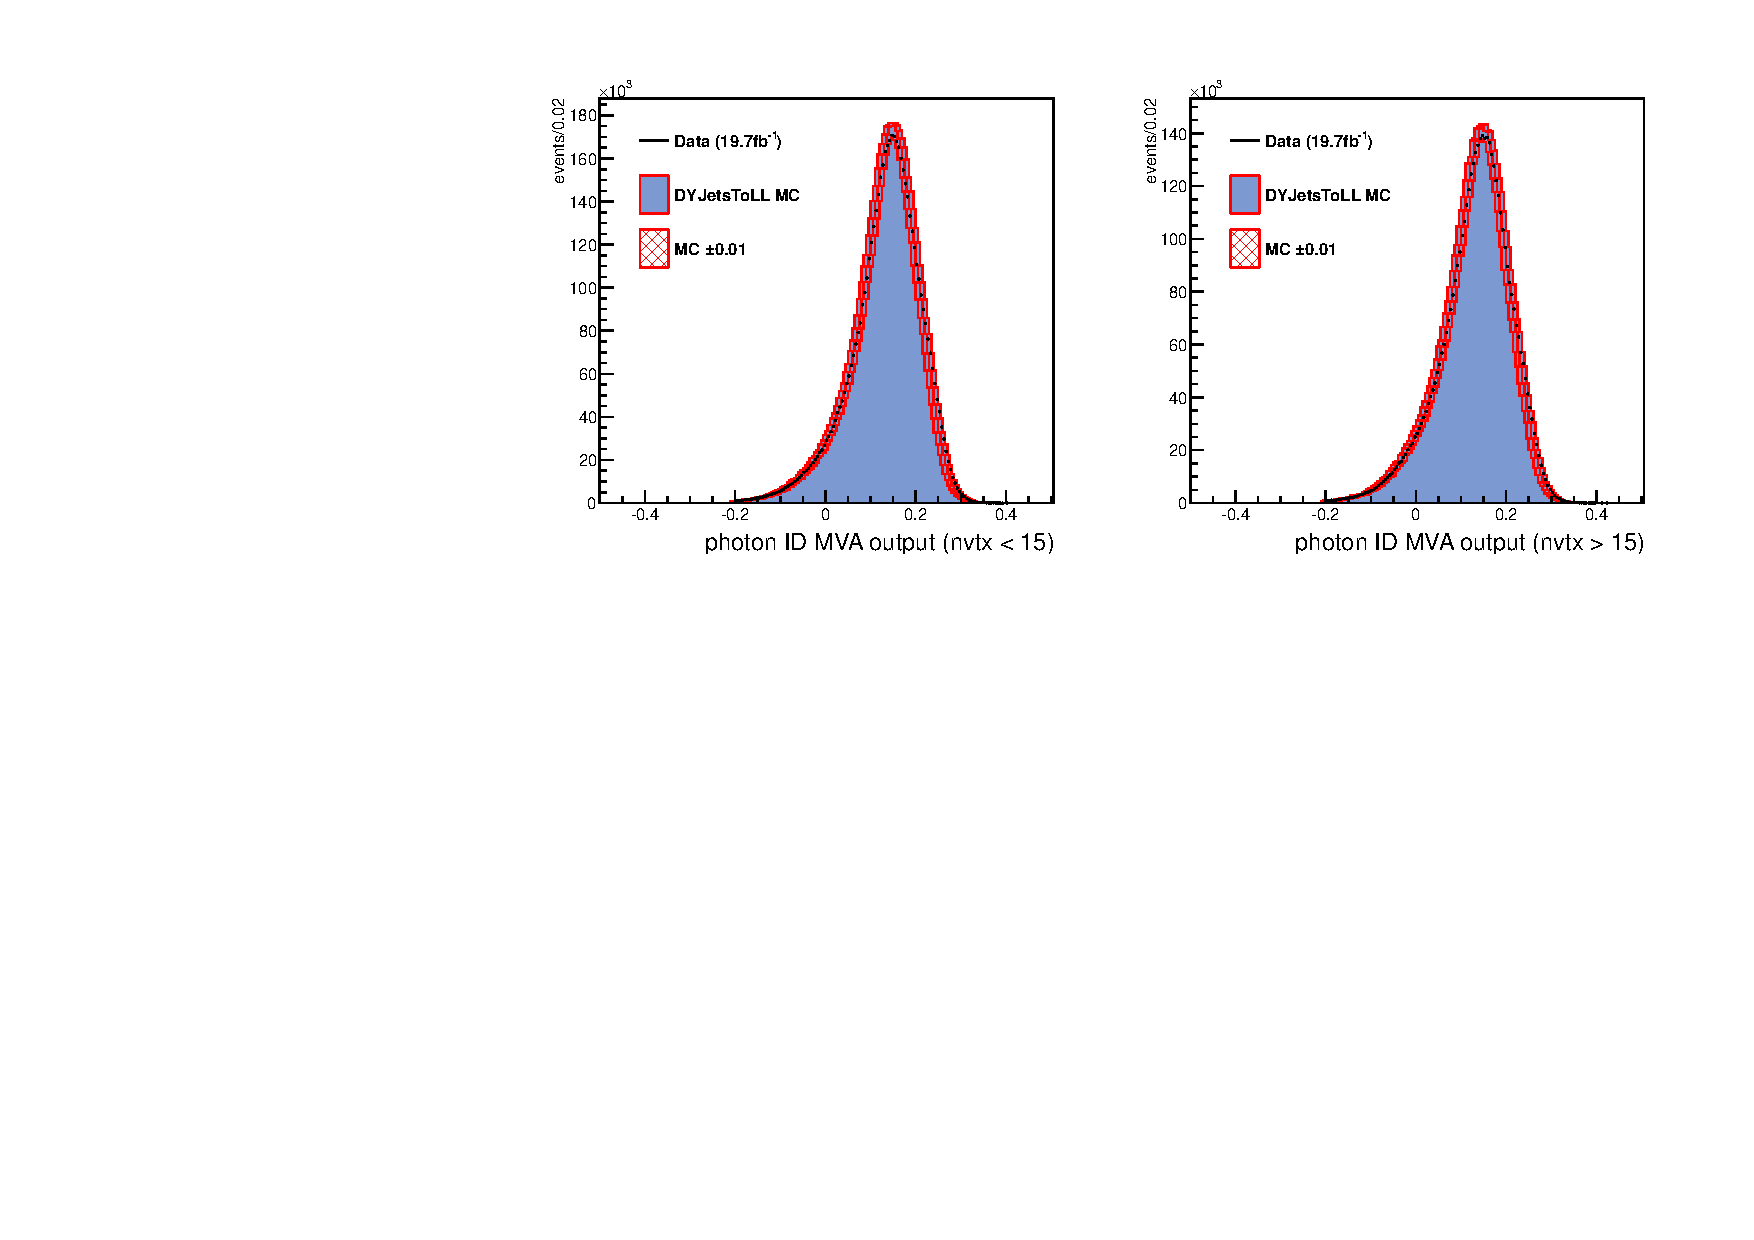
\includegraphics[width=0.48\textwidth]{selec_and_cats/plots/photonID_zee_8TeV.pdf}
  \caption{The output distribution of the photon identification \BDT for the 8~\TeV training as validated by the \Zee decay. The data is shown as the black points with the \MC as the blue histogram. The systematic uncertainty on the output as applied to the \MC is shown as the red band. \red{This is literally just a place holder for the plot that I want to show.}}
  \label{fig:photon_id_zee}
\end{figure}

\subsection{Diphoton event level MVA}
\label{sec:diphoton_bdt}

Whilst the CiC analysis selects events based on photon identification, the \MVA analysis approach is to first select photons using the photon identification \BDT described in the section above and then pass all the relevant event information through an event level \BDT. The event level classifier, referred to as the diphoton \BDT, is constructed to give a high score to events which fulfill the following criteria:

\begin{enumerate}
  \item The event kinematics should be compatible with a Higgs decay.
  \item The event has good mass resolution.
  \item The event contains two ``high quality" photons (i.e.~they have a high score from the photon ID \BDT).
\end{enumerate}

It is highly important that the \BDT is completely independent of Higgs mass and that the input variables have no, or at the least very little, dependence on the Higgs mass. This is essential to have a fair training. For example if the \BDT included the Higgs mass, or a variable highly correlated with it, it would preferentially select events with this mass therefore biasing the selection towards events which have a mass near the mass of the signal used to train with. The input variables used are,

\noindent\textbf{Event kinematics}
\begin{itemize}
  \item $p_{T}^{1(2)}/m_{\gamma\gamma}$ - The mass relative transverse momenta of each photon.
  \item $\eta^{1(2)}$ - The pseudorapidity of each photon.
  \item $\cos(\phi_{1}-\phi_{2})$ - The cosine of the angle between the two photons in the transverse plane. This variable reflects the \pT of the diphoton system (in other words the reconstructed Higgs candidate) without introducing a mass dependence.
\end{itemize}

\noindent\textbf{Mass resolution}
\begin{itemize}
  \item $\sigma_{m}^{right}/m_{\gamma\gamma}$ - The mass resolution of the event assuming the correct primary vertex has been selected. In this case the angular resolution is neglible so the variable is caluclated using just the two photon energy resolution values as,
    \begin{equation}
      \frac{\sigma_{m}^{right}}{m_{\gamma\gamma}} = \frac{1}{2}\Bigl(\frac{\sigma_{E_{1}}}{E_{1}} \oplus \frac{\sigma_{E_{2}}}{E_{2}}\Bigr).
    \end{equation}
  \item $\sigma_{m}^{wrong}/m_{\gamma\gamma}$ - The mass resolution of the event assuming the wrong vertex is selected. The vertex position in $z$ is distributed as a Gaussian with a width equivalent to $\sqrt{2}\sigma_{z}^{beamspot}$ and so the angular resolution $\sigma_{m}^{vtx}$ can be analytically calculated given the \ECAL impact positions of the two photons. Consequently the wrong vertex variable is calculated as,
    \begin{equation}
      \frac{\sigma_{m}^{wrong}}{m_{\gamma\gamma}} = \frac{\sigma_{m}^{right}}{m_{\gamma\gamma}} \oplus \frac{\sigma_{m}^{vtx}}{m_{\gamma\gamma}}.
    \end{equation}
  \item $p_{vtx}$ - The probability that the selected primary vertex is correct. In order to tie together the mass resolution information given the right vertex hypothesis and the wrong vertex hypothesis, the probability that the vertex is correct is used in addition.
  \item It is also important to specify in the training that the signal to background ratio is inversely proportional to the mass resolution. Accordingly the signal events in the training are weighted by a factor,
    \begin{equation}
      w = \frac{p_{vtx}}{\sigma_{m}^{right}/m_{\gamma\gamma}} + \frac{1-p_{vtx}}{\sigma_{m}^{wrong}/m_{\gamma\gamma}}.
    \end{equation}
\end{itemize}

\noindent\textbf{Photon quality}
\begin{itemize}
  \item $phoID^{1(2)}$ - The photon ID \BDT output value of each photon.
\end{itemize}

The training is performed separately for 7 and 8~\TeV and the samples used for the signal are all of the \SM \Hgg \MC samples (\ggH, \VBF, \VH, \ttH) appropriately weighted by cross section and the samples used for the background are the cross section weighted mixture of \SM backgrounds which include contributions from $pp\rightarrow\gamma\gamma$ (prompt-prompt), $pp\rightarrow\gamma+\mathrm{jet}$ (prompt-fake) and $pp\rightarrow\mathrm{jet+jet}$ (fake-fake) as described in Sec.~\ref{sec:mc}. The training is performed on only half of the event samples (selected by even event number) so that the BDT response can be tested on the other half (selected by odd event number).

A cut is placed on the \BDT response in order to remove almost all the events which contain two fake photons. The remaining events which pass this cut are categorised in coarse bins based the on the \BDT response. The strategy for optimising this cut value and the category boundaries is explained in Section.~\ref{sec:categorisation}. The \BDT response in data, background and signal is shown in Figure~\ref{fig:dipho_bdt}. The cut values are $>0.19$ for the 7~\TeV training and $>-0.78$ for the 8~\TeV training. It can be seen from this figure that the cut on the event level \BDT removes nearly all of the fake-fake contribution to the background whilst the remainder consists of about 70\% prompt-prompt and 30\% prompt-fake.

\begin{figure}
  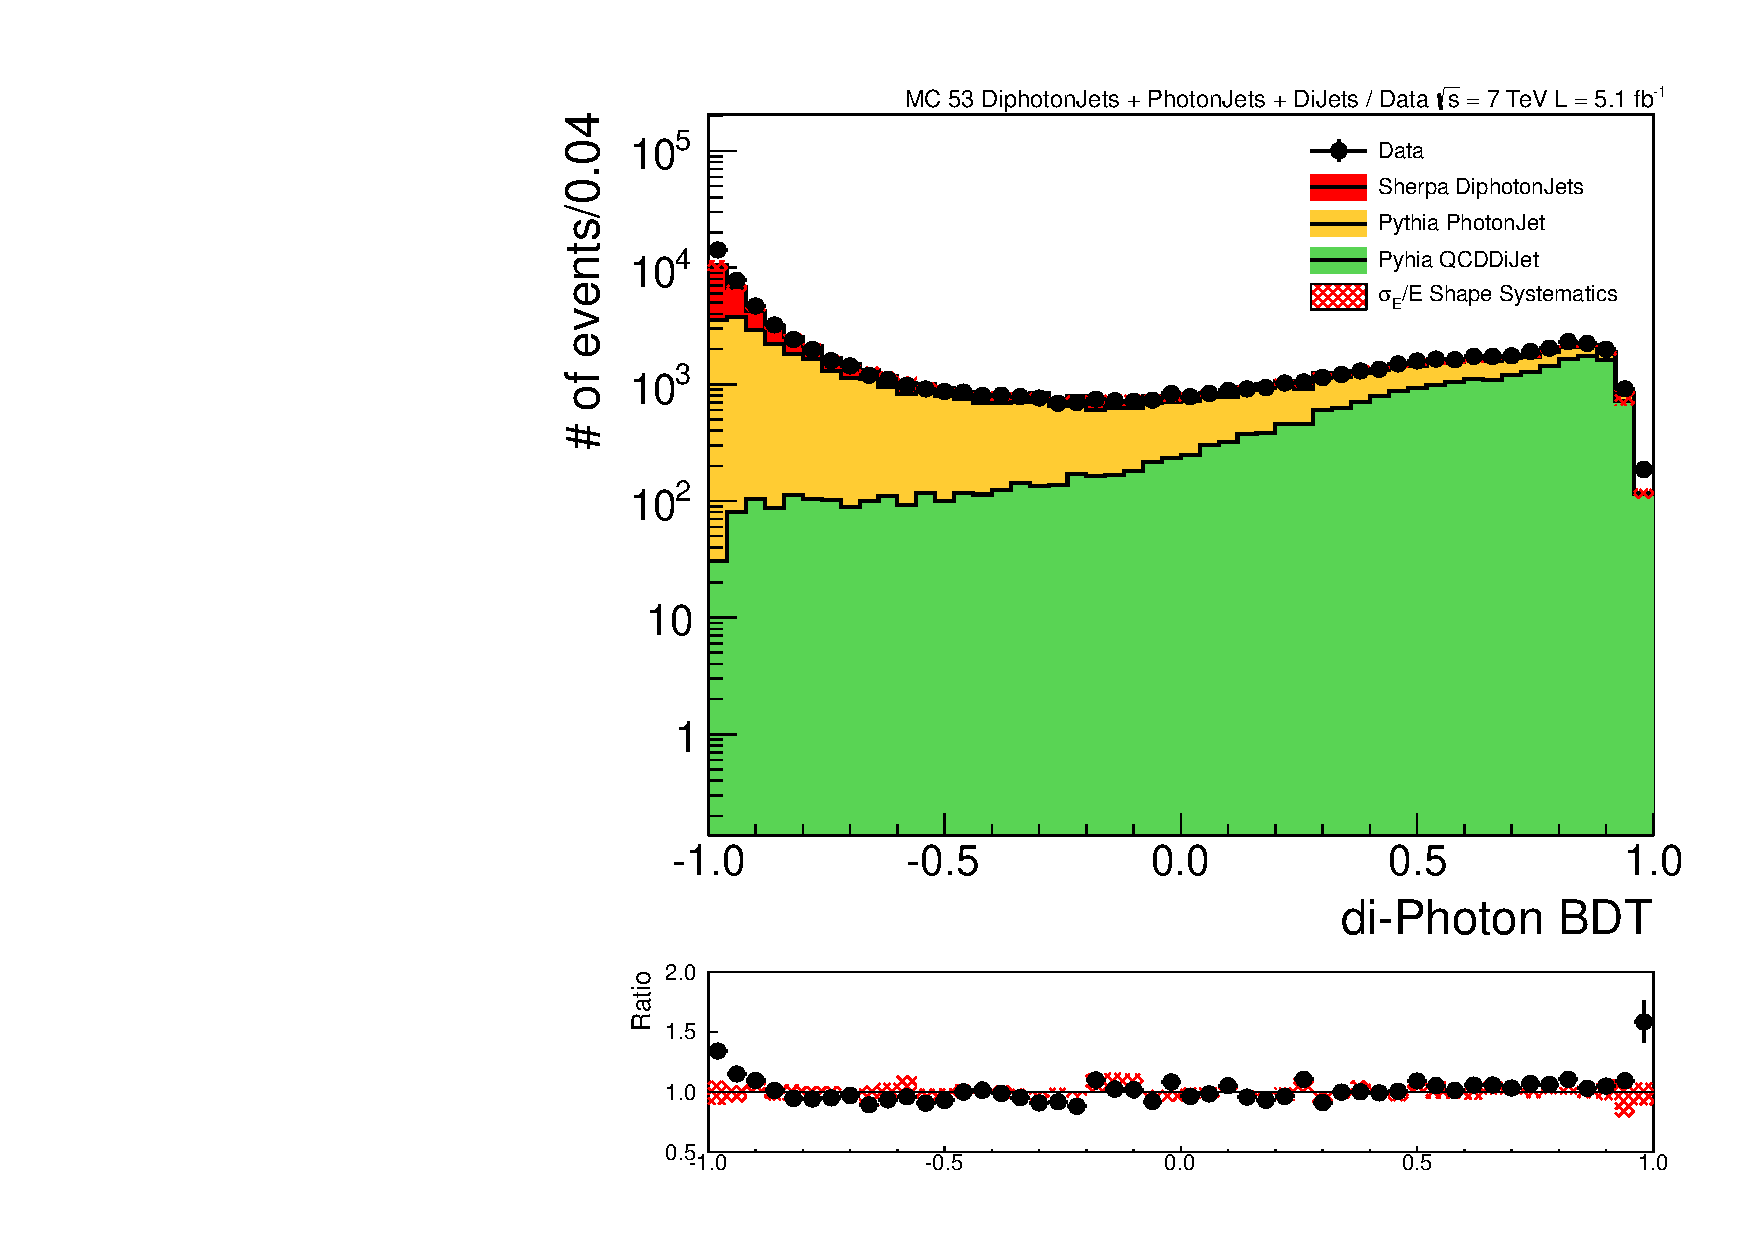
\includegraphics[width=0.48\textwidth]{selec_and_cats/plots/diphoBDT_7TeV_bkg.pdf}
  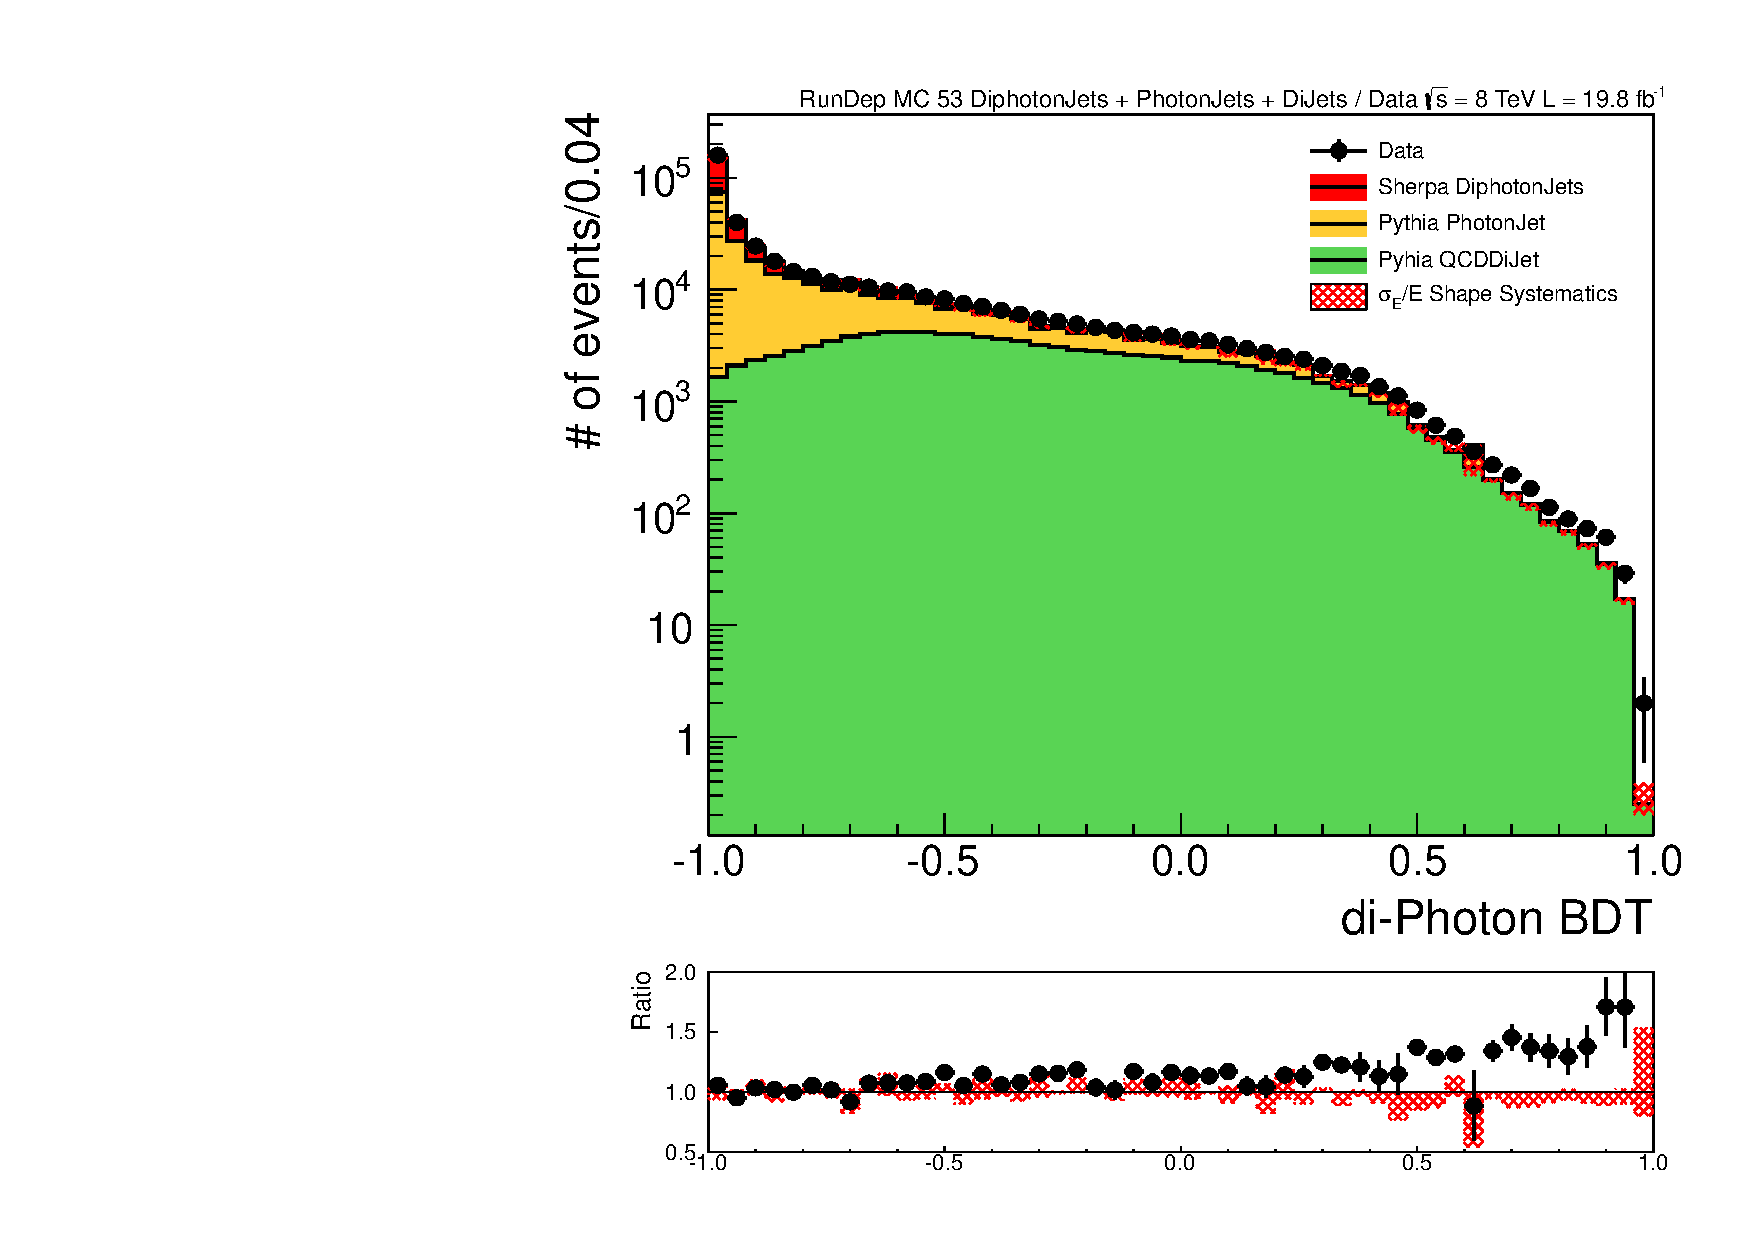
\includegraphics[width=0.48\textwidth]{selec_and_cats/plots/diphoBDT_8TeV_bkg.pdf} \\
  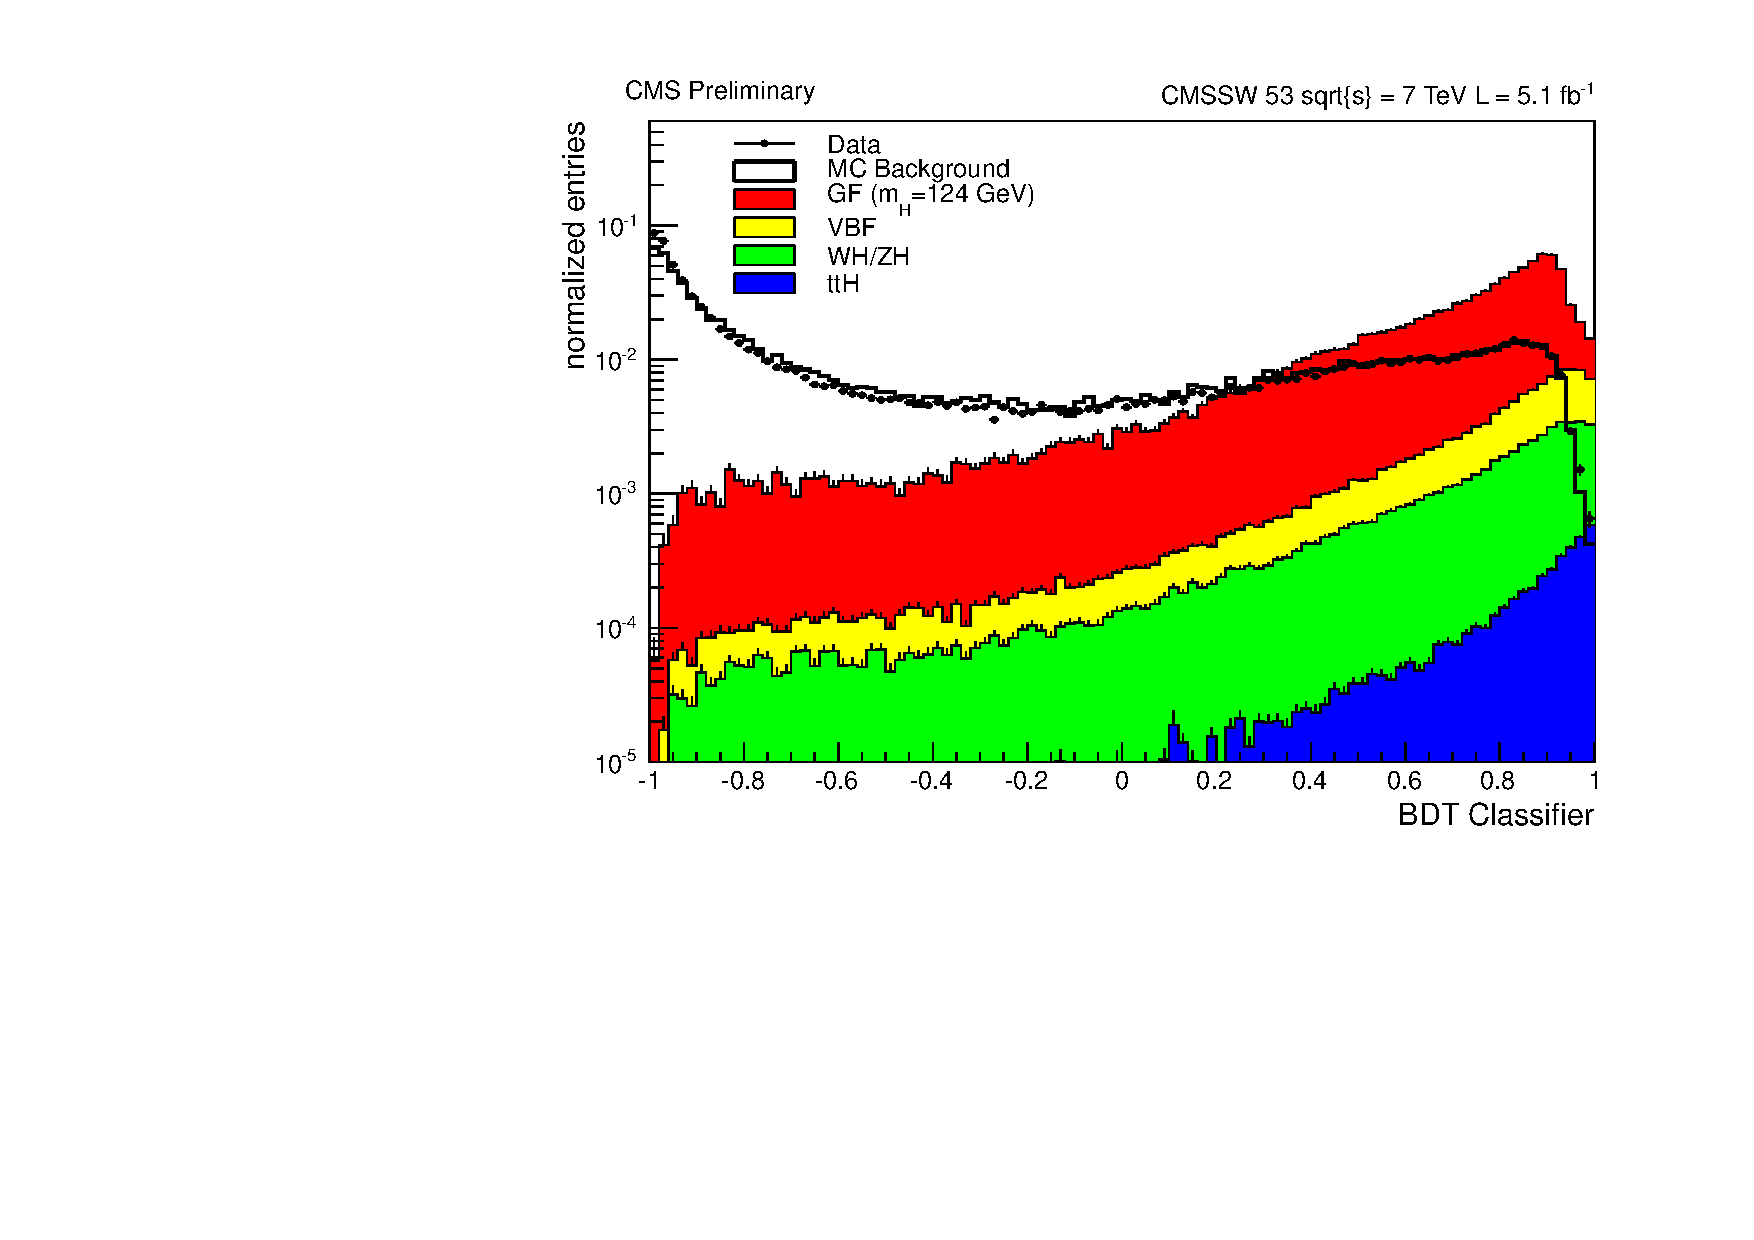
\includegraphics[width=0.48\textwidth]{selec_and_cats/plots/diphoBDT_7TeV_sig.pdf} 
  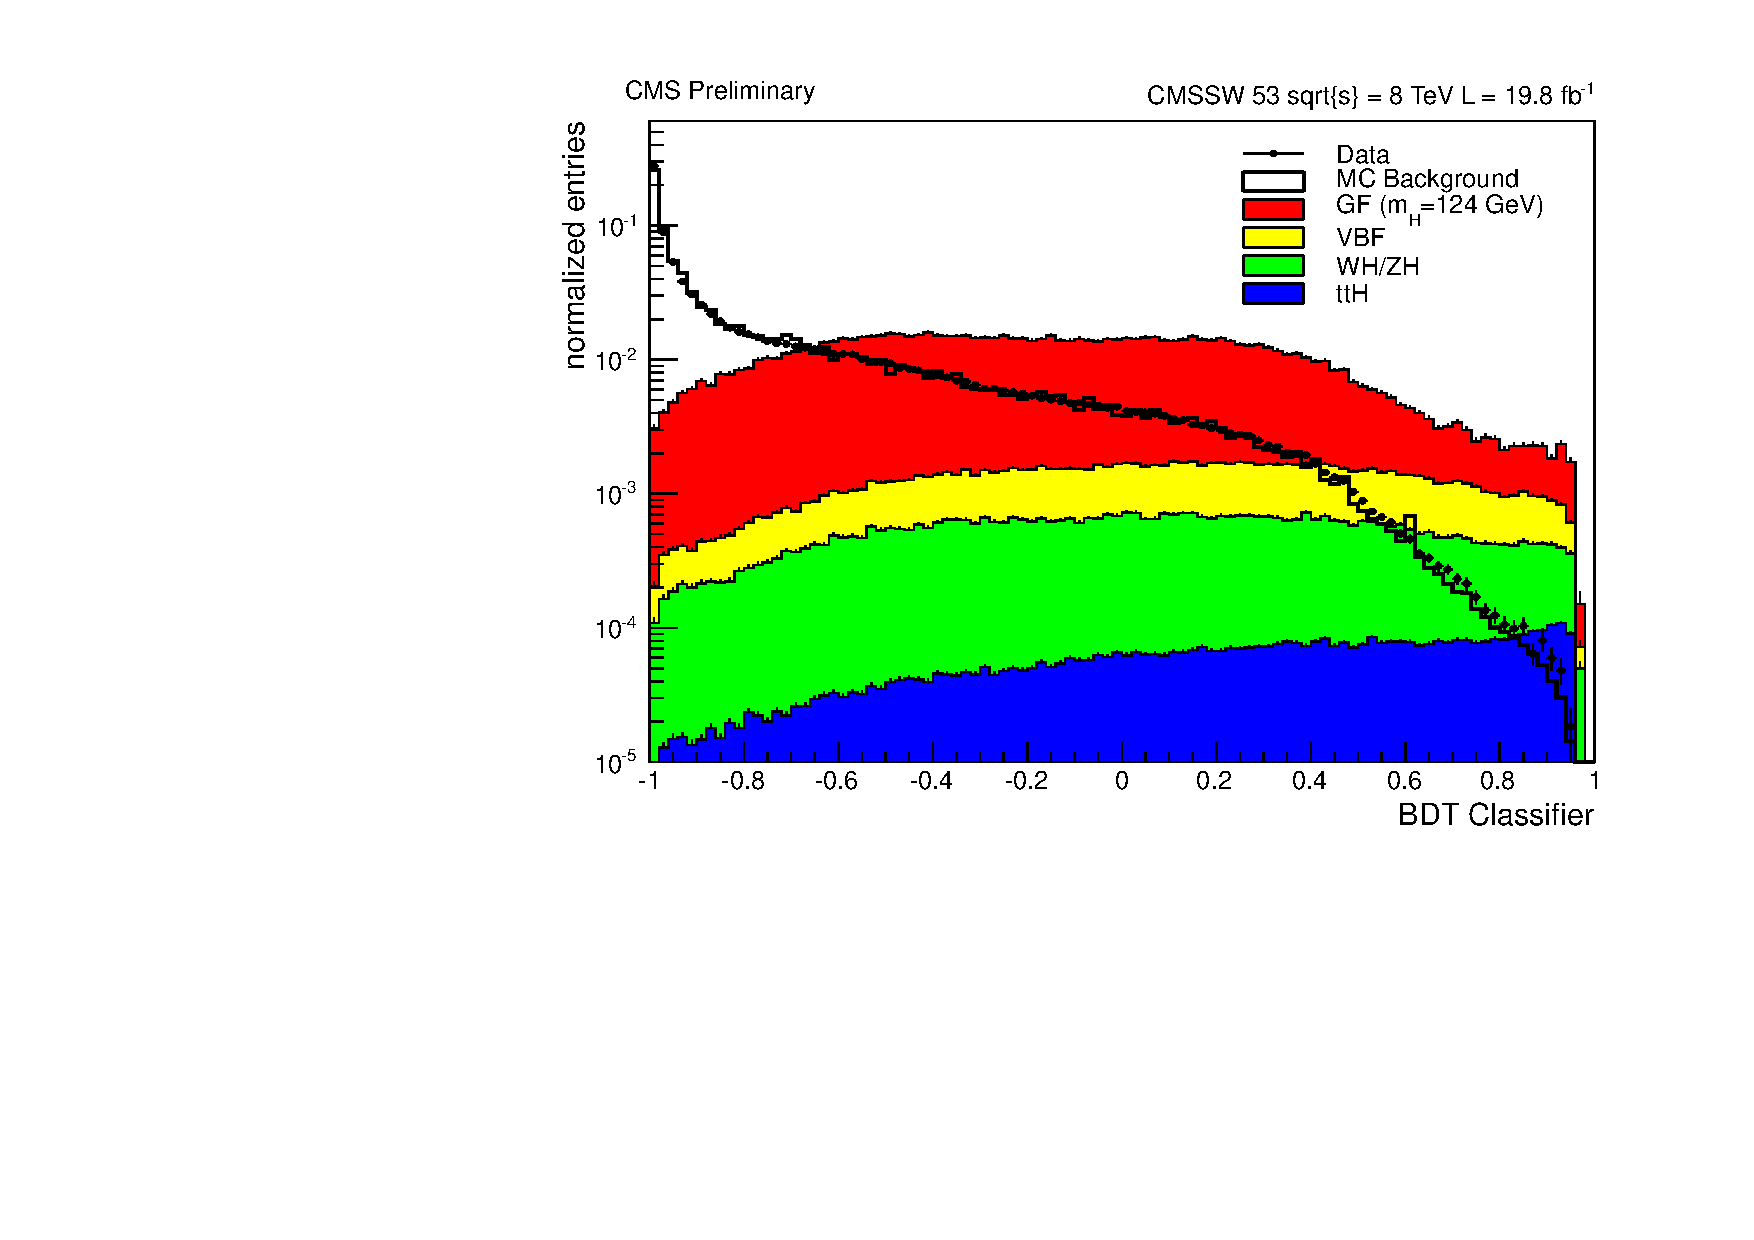
\includegraphics[width=0.48\textwidth]{selec_and_cats/plots/diphoBDT_8TeV_sig.pdf}
  \caption{The diphoton BDT response for the 7~\TeV training (left column) and 8~\TeV training (right column). The data and background distributions are shown in the plots on the top row for data in the range $100 < m_{\gamma\gamma} < 120$~\GeV and $130 < m_{\gamma\gamma} < 180$~\GeV (black points) and for the prompt-prompt background (green), prompt-fake background (yellow) and fake-fake background (red). The signal distributions are shown in the plots on the bottom row for gluon fusion (red), vector boson fusion (yellow), associated $W$, $Z$ production (green) and associated $t\bar{t}$ production (blue) alongside the data in the range $100 < m_{\gamma\gamma} < 120$~\GeV and $130 < m_{\gamma\gamma} < 180$~\GeV (black points) and the total background (hollow histogram). \red{PLOTS NEED UPDATING}}
  \label{fig:dipho_bdt}
\end{figure}

Whilst the background in this analysis is obtained in a completely data driven way the signal model is obtained from \MC. Consequently any uncertainties which effect the shape of the output distribution of this \BDT in the signal result in event migrations between the final analysis categories. The input variables whose uncertainties have the largest effect on the \BDT response in signal are the photon ID quality and the photon energy resolution estimate. This is because these variables have both i) relatively large uncertainties because of imperfect detector response modelling in the simulation and ii) are highly discriminative and hence can have a relatively large impact on the \BDT response. As these variables both vary monotonically with the \BDT response the sytematic uncertainty on them is propagated through the analysis as an event migration. Systematic uncertainties are described in more detail in Sec.~\ref{sec:systematics}. The size of this effect is shown in the \BDT response validation plot with the \Zee decay in Figure~\ref{fig:diphotonBDT_zee}. Validation plots using the \Zee channel for each of the event level \BDT input variables is shown in Appendix~\ref{app:diphoton_bdt} (\red{may not be necessary}).

\begin{figure}
  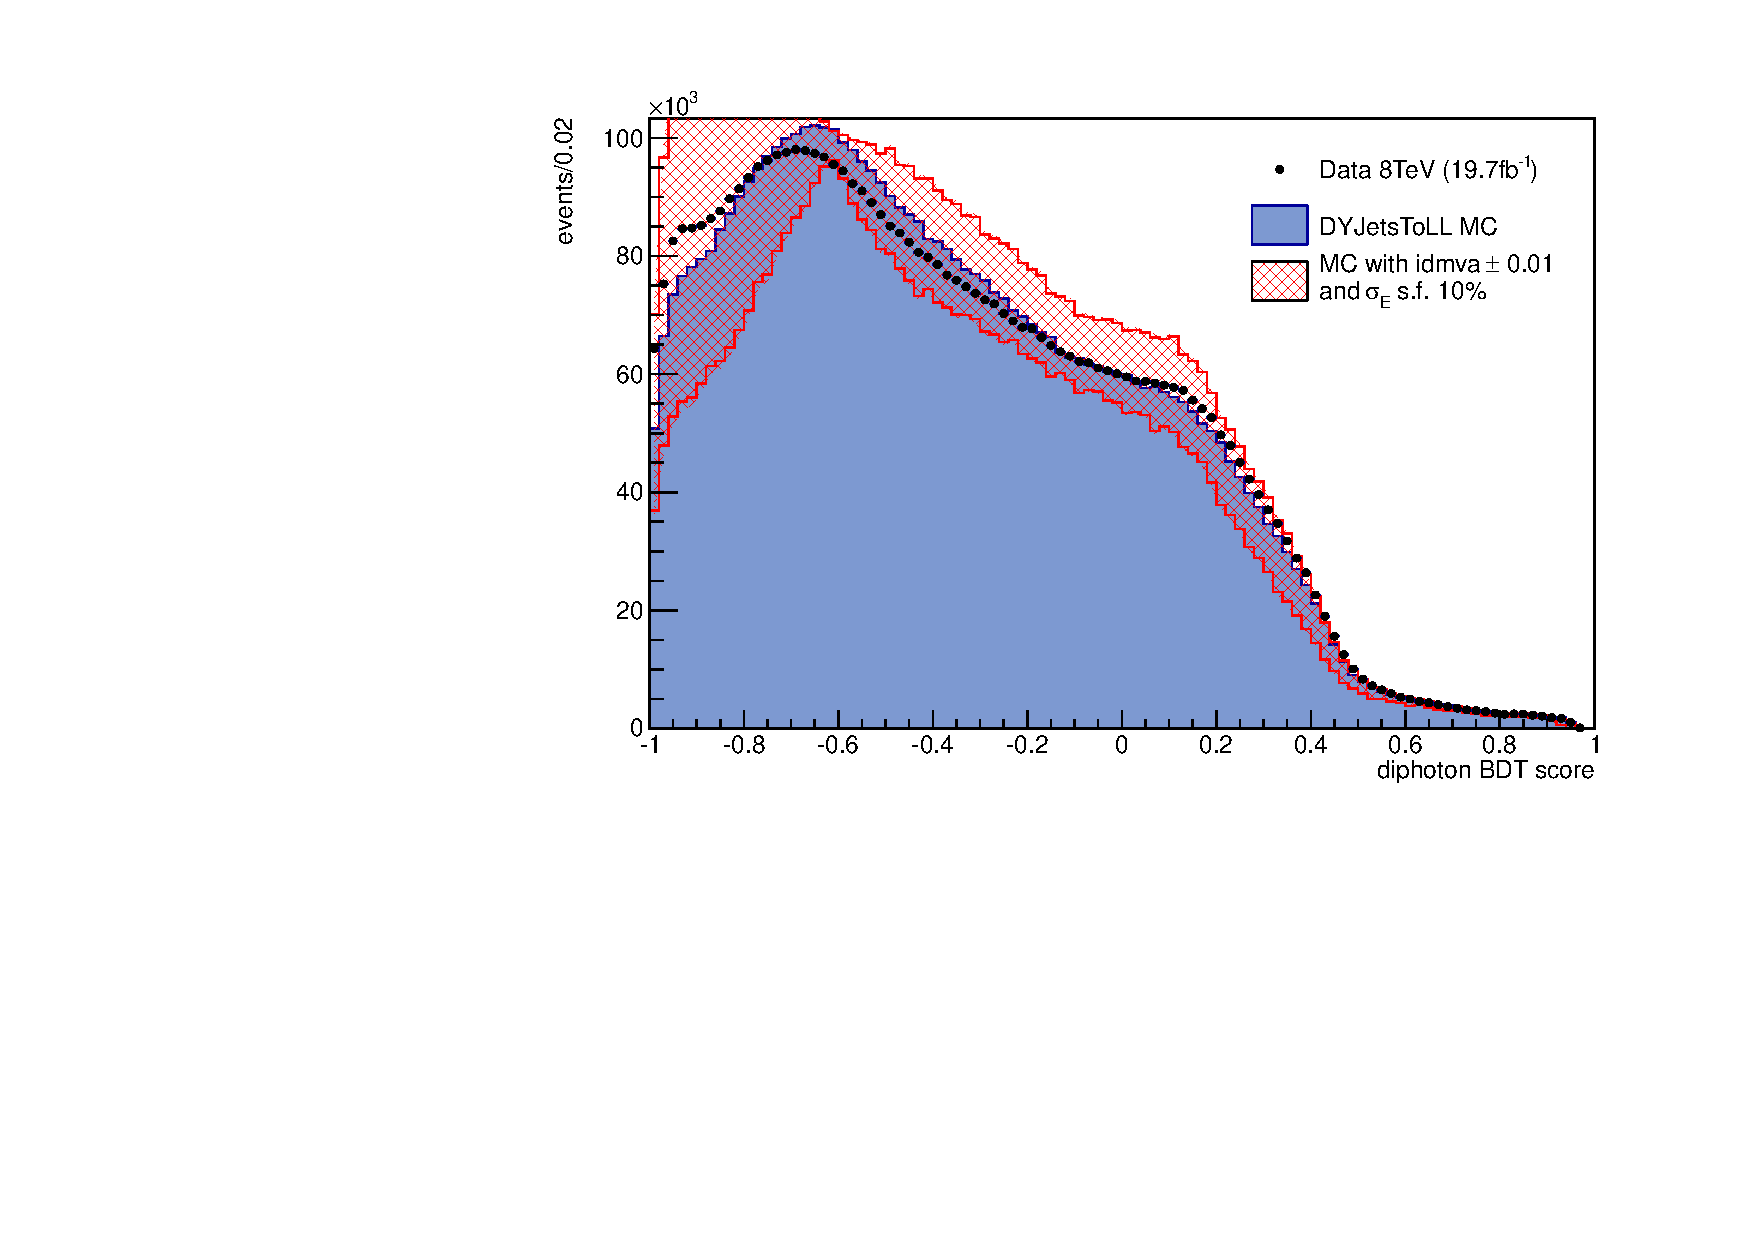
\includegraphics[width=0.6\textwidth]{selec_and_cats/plots/diphoBDT_8TeV_zee.pdf}
  \caption{The diphoton BDT response for the 8~\TeV training in the \Zee decay. The data is shown as the black points and the \MC as the blue histogram. The systematic applied to account for variation in the BDT response from mismodelling in the photon quality response and the photon energy resolution estimate are shown as the red band. \red{This is just a placeholder for the plot I want to show}}
  \label{fig:diphotonBDT_zee}
\end{figure}

% ---- SECTION ----
\section{Event categorisation}
\label{sec:categorisation}

In order to exploit different regions of phase space with similar signal to background ratios the events are split into categories. Furthermore, additional categories can be designed to enrich the selection with events characteristic of particular Higgs production modes. The \VBF production mode is typically accompanied by a pair of jets with a large pseduorapidity separation, the \VH production, which includes contributions from \WH and \ZH, may be accompanied by a charged lepton, missing transverse energy or jets originating from the decay of the associated $W$ or $Z$ boson. Similarly, \ttH production may be accompanied by b-quarks and or charged leptons. The predominant production mode, which accounts for about 88\% of the signal, is \ggH which is inclusive. The amount of signal produced from exclusive modes is approximately 8\% for \VBF, 4\% for \VH and $<$1\% for \ttH. By including a series of event tags, and separating events accordingly, all four production modes of the Higgs at the \LHC are harnessed in this analysis. This not only helps to increase the overall sensitivty to a \SM Higgs boson (given the very low background rates expected for the exclusive modes) but also significantly helps to reduce the error on measurements of the observed bosons respective couplings with fermions and bosons as the signal from the relative production modes gets split into distinct categories. The inclusive mode categorisation is done differently for each of the three analyses, a summary of all the event classifications is given in Table~\ref{tab:cat_summary} at the end of the chapter.

\subsection{Exclusive mode tagging}
\label{sec:exclusive_tags}
All events which make it to this stage will have passed the photon preselection (Sec.~\ref{sec:photon_presel}), as well as the basic requirement of two high \pT photons with $100<m_{\gamma\gamma}<180$ (Sec.~\ref{sec:event_selection}), and either the CiC selection (Sec.~\ref{sec:cic}) or the MVA selection (Sec.~\ref{sec:diphoton_bdt}) and these make up the final event sample. They now pass through the ``tagging" procedure described below in which they are organised into a set of non overlapping event classes. The tagging is done in a specific order to ensure there is no overlap between classes and the order is chosen such that preference is given to categories with a higher expected signal to background ratio. This order is shown alongside a summary of the relevant cut values in Table~\ref{tab:cat_summary} at the end of the chapter. The dijet selection for the \MVA analyses uses a specific combined dijet-diphoton \BDT to exploit the very particular kinematic properties of \VBF whereas for the \CiC analysis this is left as a cut based criteria. If an event does not meet the requirements of a particular tag it is passed onto the next tag and if it fails all tag requirements it is placed in one of the inclusive categories, whose structure is described below (Secs.~\ref{sec:inclusive_cats_cic}-~\ref{sec:inclusive_cats_sideband}), meaning that no event can now not be included in the analysis. 

\subsubsection{Dijet tagged categories for VBF}
\label{sec:vbf_tag}

The following variables are used to exploit the specific topolgy of the jet pairs associated to \VBF Higgs production,

\begin{itemize}
  \item $p_{T}^{\gamma}/m_{\gamma\gamma}$ - The mass relative transverse momenta of the leading and subleading photons,
  \item $p_{T}^{\mathrm{j}}/m_{\gamma\gamma}$ - The mass relative transverse momenta of the leading and subleading jets,
  \item $m_{\mathrm{jj}}$ - The dijet invariant mass,
  \item $\Delta\eta_{\mathrm{j}_{1}\mathrm{j}_{2}}$ - The pseduorapidity difference between the two jets.
  \item $Z = \eta(\gamma_{1}+\gamma_{2}) - \bigl(\eta(\mathrm{j}_{1})+\eta(\mathrm{j}_{2})\bigr)/2$ - The so called \emph{Zeppenfeld} variable~\cite{Zeppenfeld},
  \item $\Delta\phi_{\mathrm{j}_{1}\mathrm{j}_{2}}$ - The angular difference between the two jets in the transverse plane.
\end{itemize}

Additionally the leading photon \pT requirement is raised to $p_{T}^{\gamma_{1}}>m_{\gamma\gamma}/2$. The energy measurement of jets in the event are calibrated to correct for detector effects~\cite{jet_energy_corrections} and additional energy in the jets from pileup is removed using the \textsc{FastJet} jet areas technique described in~\cite{pu_jets1,pu_jets2,pu_jets3}. Jets are required to be within the pseudorapidity range, $\eta<4.7$.

For the \CiC analysis the dijet tagging is done in a cut based way and tagged events are placed into two categories as per the cuts defined in Table.~\ref{tab:cic_vbf_cuts}.

\begin{table}
\centering
\begin{tabular}{ l  c  c }
Variable  &  tight category & loose category \\
\hline
 $  p_{T}^{\gamma_{1}}/\mgg $  & $>0.5$ & $>0.5$ \\
 $  p_{T}^{\gamma_{2}} $       & $>25$ GeV     & $>25$ GeV     \\
 $  p_{T}^{\mathrm{j}_{1}} $   & $>30$ GeV     & $>30$ GeV     \\
 $  p_{T}^{\mathrm{j}_{2}} $   & $>30$ GeV     & $>20$ GeV     \\
 $  |\Delta\eta_{j_{1}j_{2}}| $& $ >3.0$       & $ >3.0$       \\
 $  |Z|$                       & $ <2.5$       & $ <2.5$       \\
 $  M_{j_{1}j_{2}}$            & $ >500$ GeV   & $ >250$ GeV   \\
 $  |\Delta\phi(\mathrm{jj},\gamma\gamma)|$   & $>2.6$ & $>2.6$ \\
\end{tabular}
\caption{Final selection cuts for the \VBF selection. Events from the first category are
  removed from the second one.}
\label{tab:cic_vbf_cuts}
\end{table}

For the \MVA analyses the dijet tagging is done with use of two additional \MVAs. The first is designed to exploit the \VBF kinematic properties and the second is used to combine this information with the diphoton \BDT. The input variables for the kinematic dijet \BDT are identical to those used in the cut-based \VBF selection where candidates are required to pass a \VBF preselection of two jets with $p_{T}^{\j_{1}}>30$~\GeV and $p_{T}^{\j_{2}}>20$~\GeV and invariant mass, \mjj$>75$~\GeV. The signal sample used for training is the \SM \MC with just \VBF production, whilst the \SM gluon fusion \MC is included as background along with the usual prompt-prompt, prompt-fake and fake-fake contributions. This helps produce an output in which a high score gives a very pure \VBF sample.

The combined dijet-diphoton \BDT has inputs of the kinematic dijet \BDT output, the diphoton \BDT output and $p_{T}^{\gamma\gamma}/m_{\gamma\gamma}$ in order to discriminate \VBF from both the other signal types and the background, utilising all the information avaiable in the event. The mass relative transverse momenta of the diphoton system, $p_{T}^{\gamma\gamma}/m_{\gamma\gamma}$, is included because of its considerable correlation with both the dijet \BDT output and the diphoton \BDT output.

One finds that the background rejection for \VBF is significantly improved by the use of the combined dijet-diphoton \BDT whilst the \VBF purity (i.e.~separation from \ggH) is not as good when collapsing the kinematic dijet \BDT and the combined \BDT into one step. Consequently the trainings are performed separately and the \VBF categories are defined by picking out regions which have a high score in the combined dijet-diphoton \BDT response. The optimisation procedure for deciding the category boundaries is analogous to the one used for the inclusive categories in the \MFM analysis where the target is to minimise the expected uncertainty of the signal strength from the \VBF process alone when moving the boundaries around. It is explained further in Section~\ref{sec:inclusive_cats_massfac}. At 8~\TeV there are three \VBF categories and at 7~\TeV there are two. The output distributions for the signal and background with the cut boundaries are shown for the two dijet \BDTs are shown in in Figures~\ref{fig:vbf_dijet_kin} and ~\ref{fig:vbf_dijet_comb}. Each successive \BDT training uses statisically independent \MC samples to avoid selection bias from fluctuations in the simulation. 

\begin{figure}
  
\includegraphics[width=0.48\textwidth]{placeholder.pdf}
  
\includegraphics[width=0.48\textwidth]{placeholder.pdf} \\
  
\includegraphics[width=0.48\textwidth]{placeholder.pdf}
  
\includegraphics[width=0.48\textwidth]{placeholder.pdf}
  \caption{The distributions of the kinematic dijet \BDT response for the \VBF signal (left) and the background (right) for the 7TeV (top row) and 8TeV (bottom row) training.}
  \label{fig:vbf_dijet_kin}
\end{figure}

\begin{figure}
  
\includegraphics[width=0.48\textwidth]{placeholder.pdf}
  
\includegraphics[width=0.48\textwidth]{placeholder.pdf} \\
  
\includegraphics[width=0.48\textwidth]{placeholder.pdf}
  
\includegraphics[width=0.48\textwidth]{placeholder.pdf}
  \caption{The distributions of the combined dijet-diphoton \BDT response for the \VBF signal (left) and the background (right) for the 7TeV (top row) and 8TeV (bottom row) training. The red dahsed lines corresponded to the location of the category boundaries.}
  \label{fig:vbf_dijet_comb}
\end{figure}

\subsubsection{Lepton, jet and \MET tagged categories for \VH}
\label{sec:vh_tag}

The selection for the four categories designed to tag \VH production are optimised by minimising the expected uncertainty on the signal strength of this process alone. Two of the classes require at least one charged muon or electron and are split into a tight selection category and a looser selection category, the third is for events consistent with large \MET and the fourth for events consistent with two or more jets. The leading photon cut is raised to $p_{T}^{\gamma_{1}}>3m_{\gamma\gamma}/8$ for the lepton and \MET tagged categories and $p_{T}^{\gamma_{1}}>m_{\gamma\gamma}/2$ for the jet tagged category. The category requirements are as follows,

\begin{itemize}
  \item \textbf{\VH Tight $l$}: The tighly selected lepton category is characterised by the signature of a leptonically decaying $W$ or $Z$ boson and as such requires the presence of \MET$>35$~\GeV or another lepton of the same flavour and opposite charge as the first. In the first case (of a lepton + \MET) the lepton is required to have $p_{T}>20$~\GeV, in the latter case (of two leptons) the requirement is $p_{T}>10$~\GeV for both leptons whilst the invariant mass of the dilepton pair must be $70 < m_{ll} < 110$~\GeV. The diphoton \BDT output is required to be $>0.1$ ($>-0.6$) for the 7 (8)~\TeV datasets.
  \item \textbf{\VH Loose $l$}: For the loosely selected lepton category the lepton \pT must satisfy $p_{T}>20$~\GeV. The selection requirements are designed to reduce the background from leptonic $Z$ bosons (not associated with a Higgs) that contain initial or final state radiation faking the diphoton signal. Consequently, leptons are required to be separated by at least $\Delta R>1.0$ from the closest photon and the invariant mass of any electron-photon pairs must be more than 10~\GeV away from the $Z$ boson mass. In addition a conversion veto is applied to the electrons to reduce the rate of misidentified photons. The diphoton \BDT output is required to be $>0.1$ ($>-0.6$) for the 7 (8)~\TeV datasets.
  \item \textbf{\VH \MET tag}: Accurate measurement and simulation of the \MET vector has been studied in detail at \CMS and a set of standard corrections (for both data and simulation) are applied~\cite{met_corrs}. The corrected \MET is required to pass \MET$>70$~\GeV whilst the angular separation in the transverse plane betwen the diphoton system and the \MET direction must pass $\Delta\phi(\gamma\gamma,\MET)>2.1$, and similarly the angle between the diphoton system and the leading jet must pass $\Delta\phi(\gamma\gamma,\mbox{jet})<2.7$. The diphoton \BDT output is required to be $>0.8$ ($>0.0$) for the 7 (8)~\TeV datasets.   
  \item \textbf{\VH jet tag}: The event must contain at least one jet pair in which both jets have $p_{T}>40$~\GeV and $|\eta|<2.4$ and have an invariant mass within the range $60<m_{jj}<120$~\GeV. The diphoton transverse momenta must satify $p_{T}^{\gamma\gamma}>13m_{\gamma\gamma}/12$. Additionally the angular correlation between the diphoton system and the dijet system from \VH associated Higgs decays can be exploited. The angle, $\theta^{\star}$, between the diphoton direction in the diphoton-dijet rest frame and the lab frame is flat for events from \VH decays whereas for the background and gluon fusion produced Higgs decays the distribution peaks at $|cos(\theta^{\star})|=1$. Consequently, there is a requirement that $|cos(\theta^{\star})|<0.5$. The diphoton \BDT output is required to be $>0.6$ ($>0.2$) for the 7 (8)~\TeV datasets. 
\end{itemize}

\subsubsection{Lepton and jet tagged categories for \ttH}
\label{sec:tth_tag}

There are two categories for tagging production from \ttH decays, one which is lepton based and one which is jet based. The total fraction of signal expected from \ttH is $<$1\% so only a handful of events are expected. Consequently for the 7~\TeV dataset the two categories are merged into one class. As for the \VH tagged categories the cuts are optimised to minimise the expected uncertainty of the signal strength measurement of the \ttH process alone.

For both classes the leading photon \pT cut is raised to $p_{T}^{\gamma_{1}}>m_{\gamma\gamma}/2$, all jets are required to have \pT$>25$~\GeV and there must be at least one b-tagged jet present. The specific requirements of each category are as follows,

\begin{itemize}
  \item \textbf{\ttH multijet tag}: The requirement is at least four additional jets in the event and no lepton. The diphoton \BDT output is required to be $>0.6$ ($>-0.2$) for the 7 (8)~\TeV datasets. 
  \item \textbf{\ttH lepton tag}: At least one more jet in the event and one muon or electron which has \pT$>20$~\GeV. The diphoton \BDT output is required to be $>0.6$ ($>-0.6$) for the 7 (8)~\TeV datasets.  
\end{itemize}

\subsection{Inclusive mode categorisation in the cut based analysis}
\label{sec:inclusive_cats_cic}

Any event which passes the cut based photon selection described in Section~\ref{sec:cic} and does not fall into one of the exclusive categories described above is split into one of eight inclusive categories depending on the supercluster position, \eta, of the two photons, the conversion variable, \rnine, of the two photons and the mass relative diphoton transverse momenta, \pToM. The categories are defined in Table~\ref{tab:cic_cats}.

\begin{table}
  \begin{center}
    \begin{tabular}{lccc}
                 & \pToM                            & Maximum \eta                                    & Minimum \rnine \\
      \hline
      Untagged 0 & \multirow{4}{*}{$>40$~\GeV}      & \multirow{2}{*}{$<$1.444}                       & $>0.94$ \\
      Untagged 1 &                                  &                                                 & $<0.94$ \\
      Untagged 2 &                                  & \multirow{2}{*}{$<$2.5}                         & $>0.94$ \\
      Untagged 3 &                                  &                                                 & $<0.94$ \\
      \hline
      Untagged 4 & \multirow{4}{*}{$<40$~\GeV}      & \multirow{2}{*}{$<$1.444}                       & $>0.94$ \\
      Untagged 5 &                                  &                                                 & $<0.94$ \\
      Untagged 6 &                                  & \multirow{2}{*}{$<$2.5}                         & $>0.94$ \\ 
      Untagged 7 &                                  &                                                 & $<0.94$ \\
    \end{tabular}
    \caption{The definition of the inclusive categories for the \CiC analysis}
    \label{tab:cic_cats}
  \end{center}
\end{table}

\subsection{Inclusive mode categorisation and VBF dijet categorisation in the mass factorised \MVA analysis}
\label{sec:inclusive_cats_massfac}

Firstly the combined dijet-diphoton \BDT score is used to define a set of \VBF categories. The goal is to find the configuration of category boundaries which minimise the expected uncertainty on the signal strength for \VBF production alone, allowing the number of categories and where the category boundaries lie to be completely free floating, with the additional requirement that the efficiency $\times$ acceptance of the categories matches between 7 and 8~\TeV. This results in a tight \VBF category for events with a very high combined dijet-diphoton \BDT score, a somewhat looser category and then one or more very loose categories. One finds that dropping the loosest category has a neglible impact ($<$1\%) on the expected uncertainty and as such the upper boundary for the loosest category is turned into a lower cut. All events which pass the \VBF preselection (described in Sec.~\ref{sec:vbf_tag}) and fail the lower cut are then classified somewhere in the inclusive categories defined below. 

Once the \VBF category boundaries have been found the same procedure is deployed using the diphoton \BDT score. This time the target is to minimise the expected uncertainty on the total signal strength, allowing the number of categories and the category boundary values to be completely free floating. One finds a rather similar structure and that dropping events in the very loosest category has a neglible impact on the performance and consequently this dictates the lower cut value for the diphoton \BDT. 

Due to the amount of simulation \MC available to do these studies the precision to which the boundary values are important is quite broad. Furthermore, the expected uncertainty minima are very shallow so the exact position of the boundaries has a very small impact on the performance of the analysis. For the 7 (8)~\TeV datasets there are 4 (5) inclusive categories with a lower diphoton \BDT cut of 0.19 (-0.78) and 2 (3) \VBF categories. The boundary optimisation procedure is pictorally represented in Figure~\ref{fig:bdt_boundaries_pic}.

\begin{figure}
  
\includegraphics[width=0.8\textwidth]{placeholder.pdf}
  \caption{A pictoral representation of how the VBF and inclusive category boundaries are optimised}
  \label{fig:bdt_boundaries_pic}
\end{figure}

\subsection{Inclusive mode categorisation in the sideband \MVA analysis}
\label{sec:inclusive_cats_sideband}

In the \SMVA analysis all the exclusive categories are identical to the \MFM analysis (including the \VBF categories). However the inclusive categorisation is done slightly differently. In the sideband analysis the signal region is defined in a $\pm2$\% window around the hypothesis Higgs mass. The analysis is performed as a cut and count in the signal window over several bins. There is one bin for each exclusive category and then several more for the inclusive. The binning scheme for the inclusive events is defined as follows,

\begin{itemize}
  \item Make two dimensional distributions of the diphoton \BDT score and the distance of the invariant mass from the hypothesised Higgs mass, $\Delta m/m_{H}$, in the $\pm2$\% window for signal and background, as shown in Figure~\ref{fig:sideband_inputs}, where,
    \begin{equation}
      \Delta m/m_{H} = \frac{m_{\gamma\gamma} - m_{H}}{m_{H}}.
    \end{equation}
  \item Select bins by isolating regions of this 2D phase space which have similar $S/B$ ratios and optimise the boundaries to give the maximum expected signal significance.   
\end{itemize}

Clearly the most sensitive bins will be the ones which have a high diphoton \BDT score and have a low value of $|\dmom|$ (i.e.\ are near the signal peak). The category boundaries in this 2D plane are shown as different shades in Figure~\ref{fig:sideband_cats}. In total there are 8 (10) inclusive bins for the 7 (8)~\TeV samples in the \SMVA.

\begin{figure}
  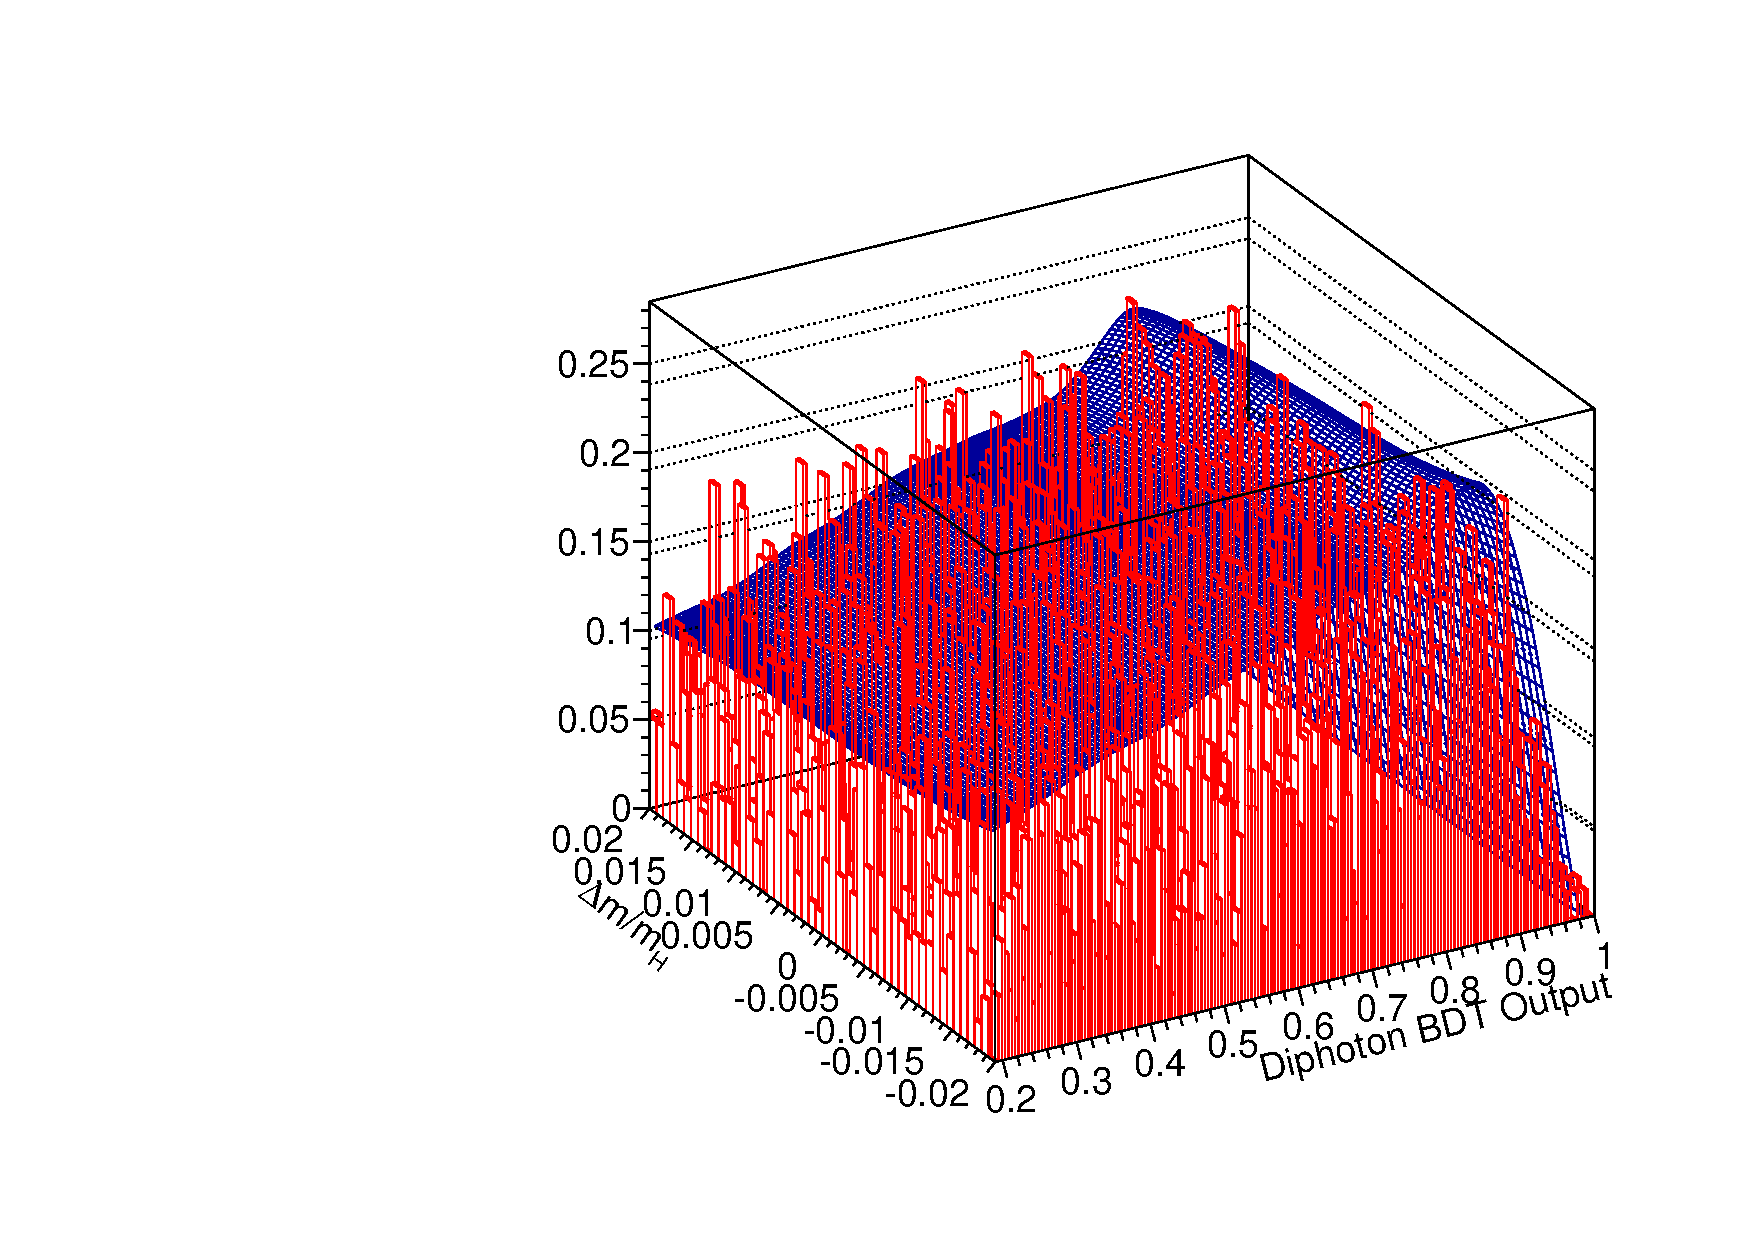
\includegraphics[width=0.48\textwidth]{selec_and_cats/plots/sideband_bkg_7TeV.pdf}
  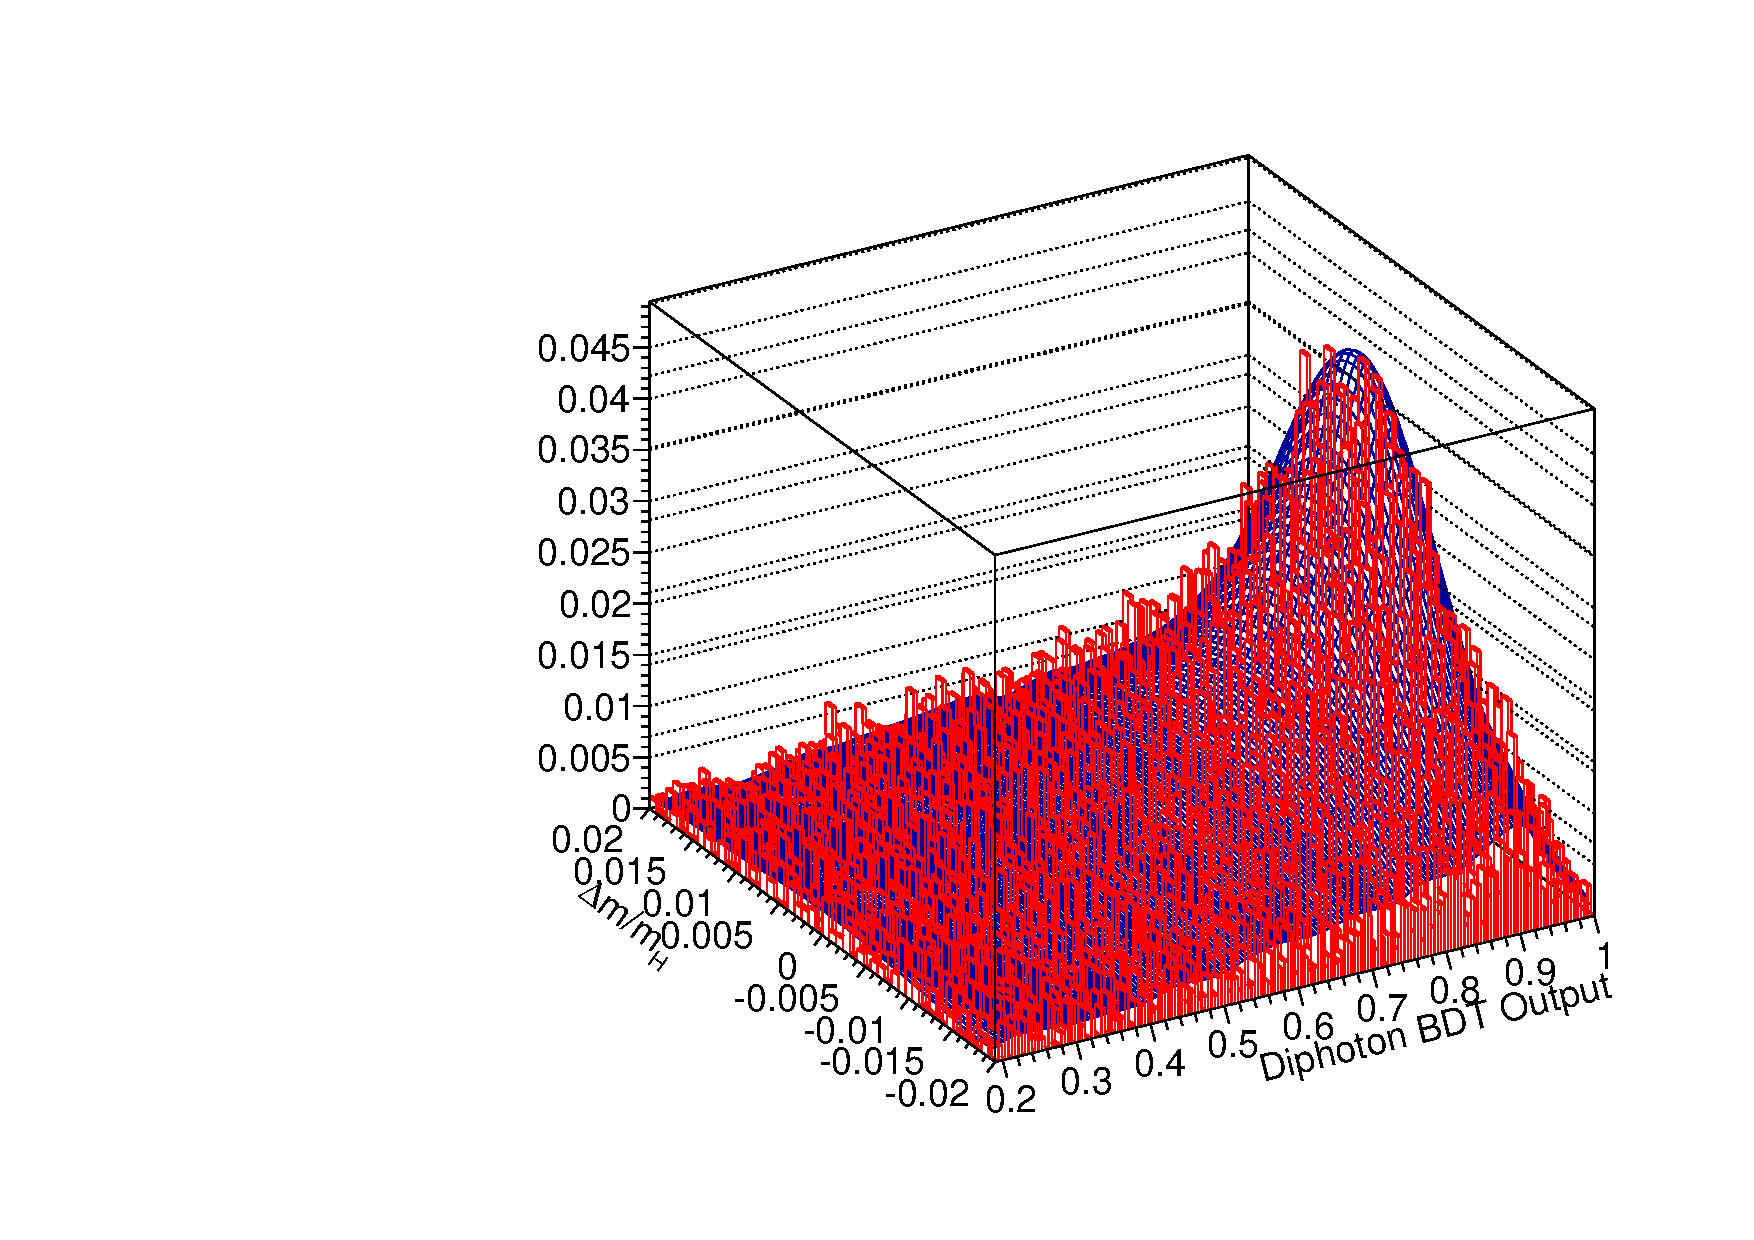
\includegraphics[width=0.48\textwidth]{selec_and_cats/plots/sideband_sig_7TeV.pdf} \\
  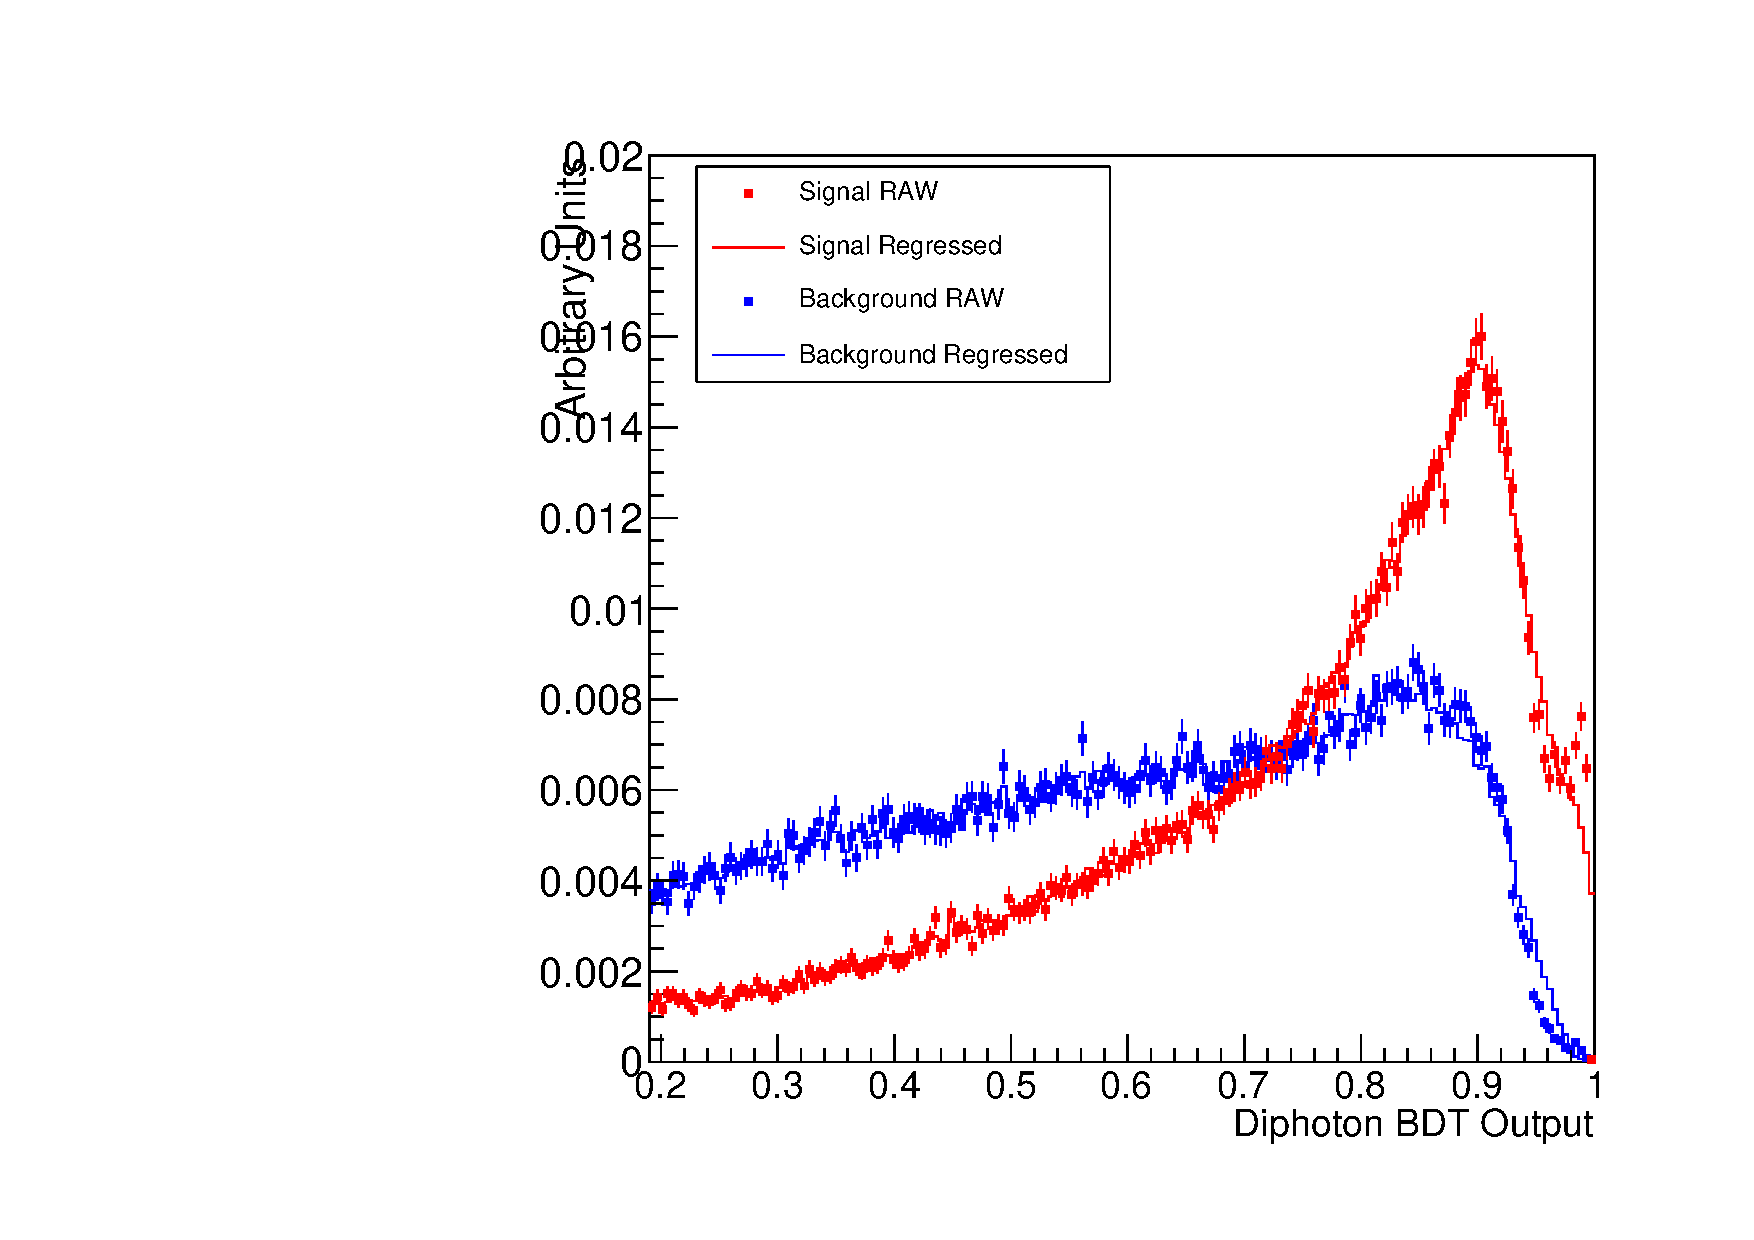
\includegraphics[width=0.48\textwidth]{selec_and_cats/plots/sideband_diphobdt_7TeV.pdf}
  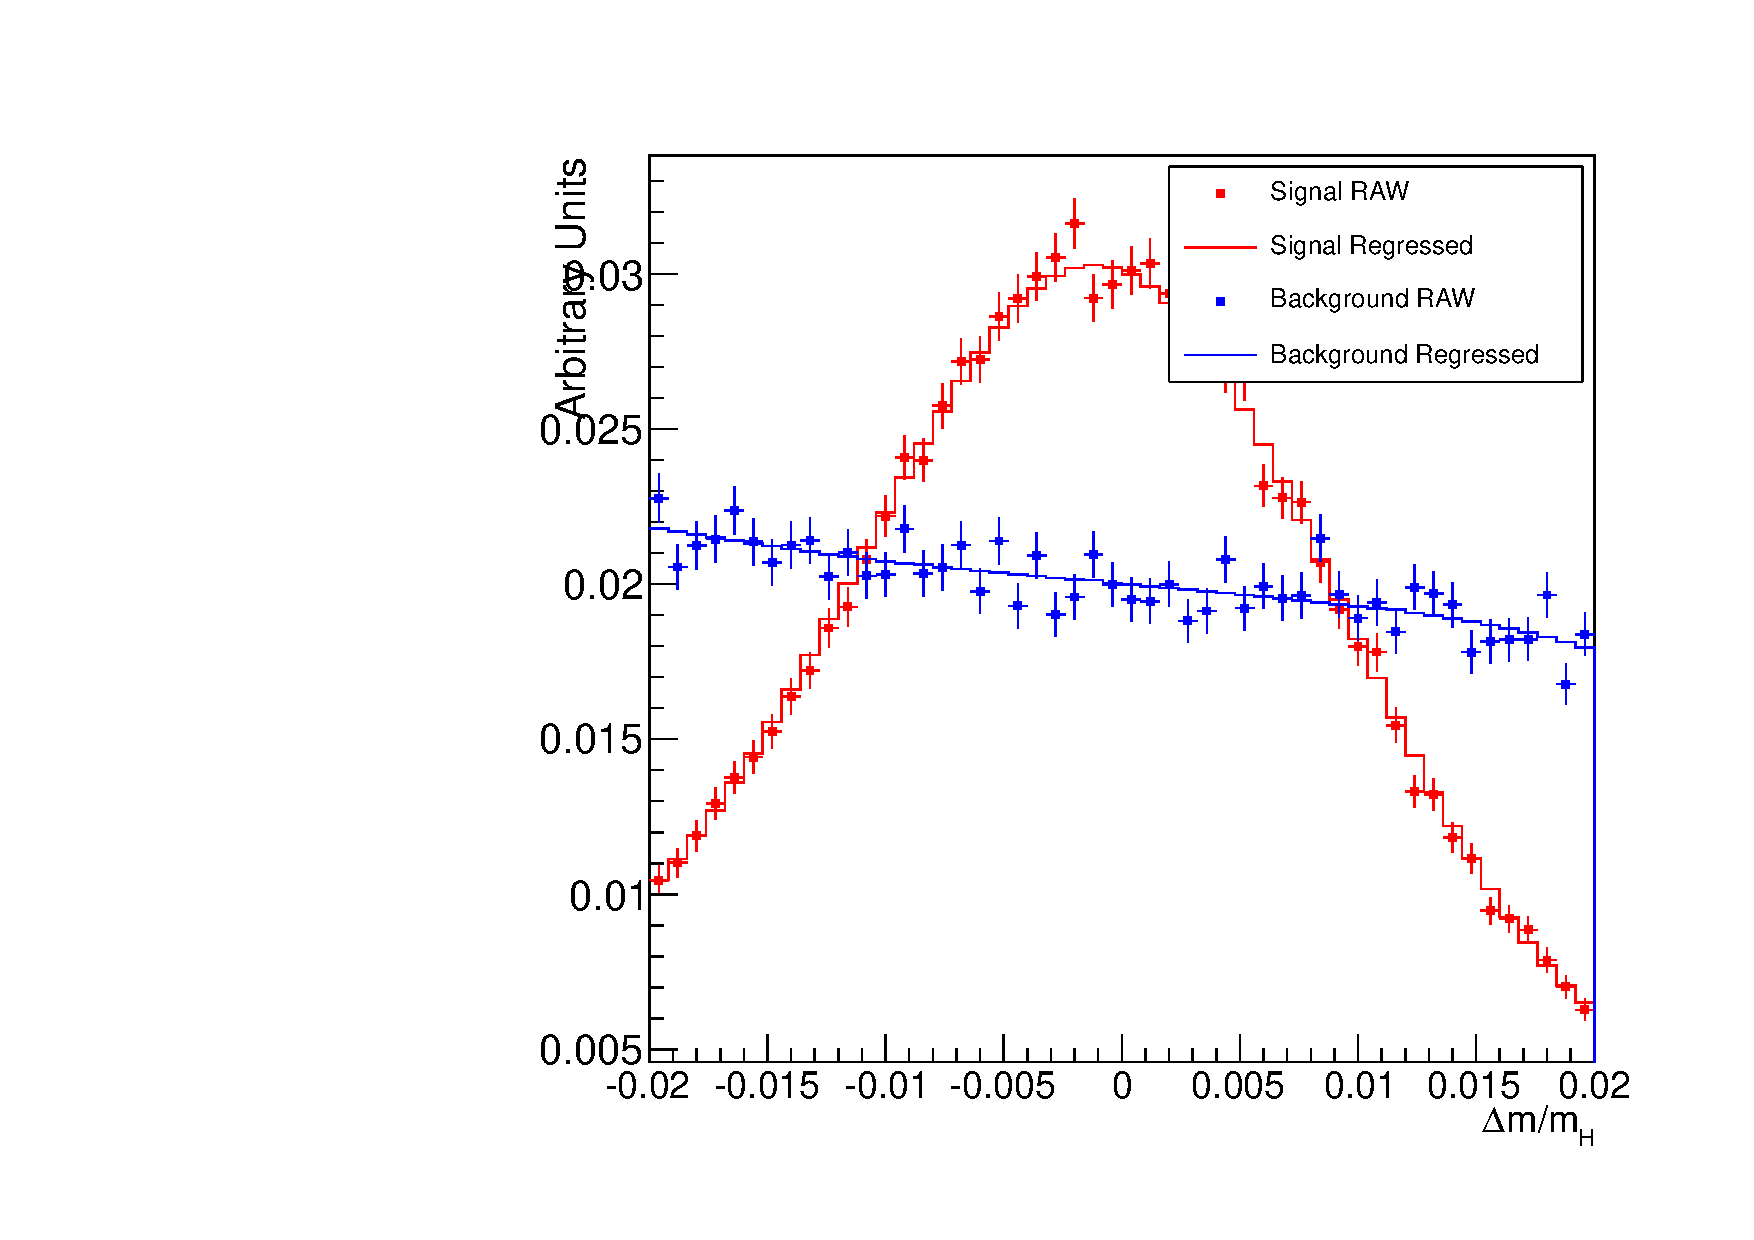
\includegraphics[width=0.48\textwidth]{selec_and_cats/plots/sideband_dmom_7TeV.pdf} \\
  \caption{Two dimensional distributions of the diphoton \BDT output and \dmom are shown on the top row for the background (left) and signal (right) for the 7~\TeV sample. The bottom rows show the projection for signal (red) and background (blue) in the two variables.}
  \label{fig:sideband_inputs}
\end{figure}

\begin{figure}
  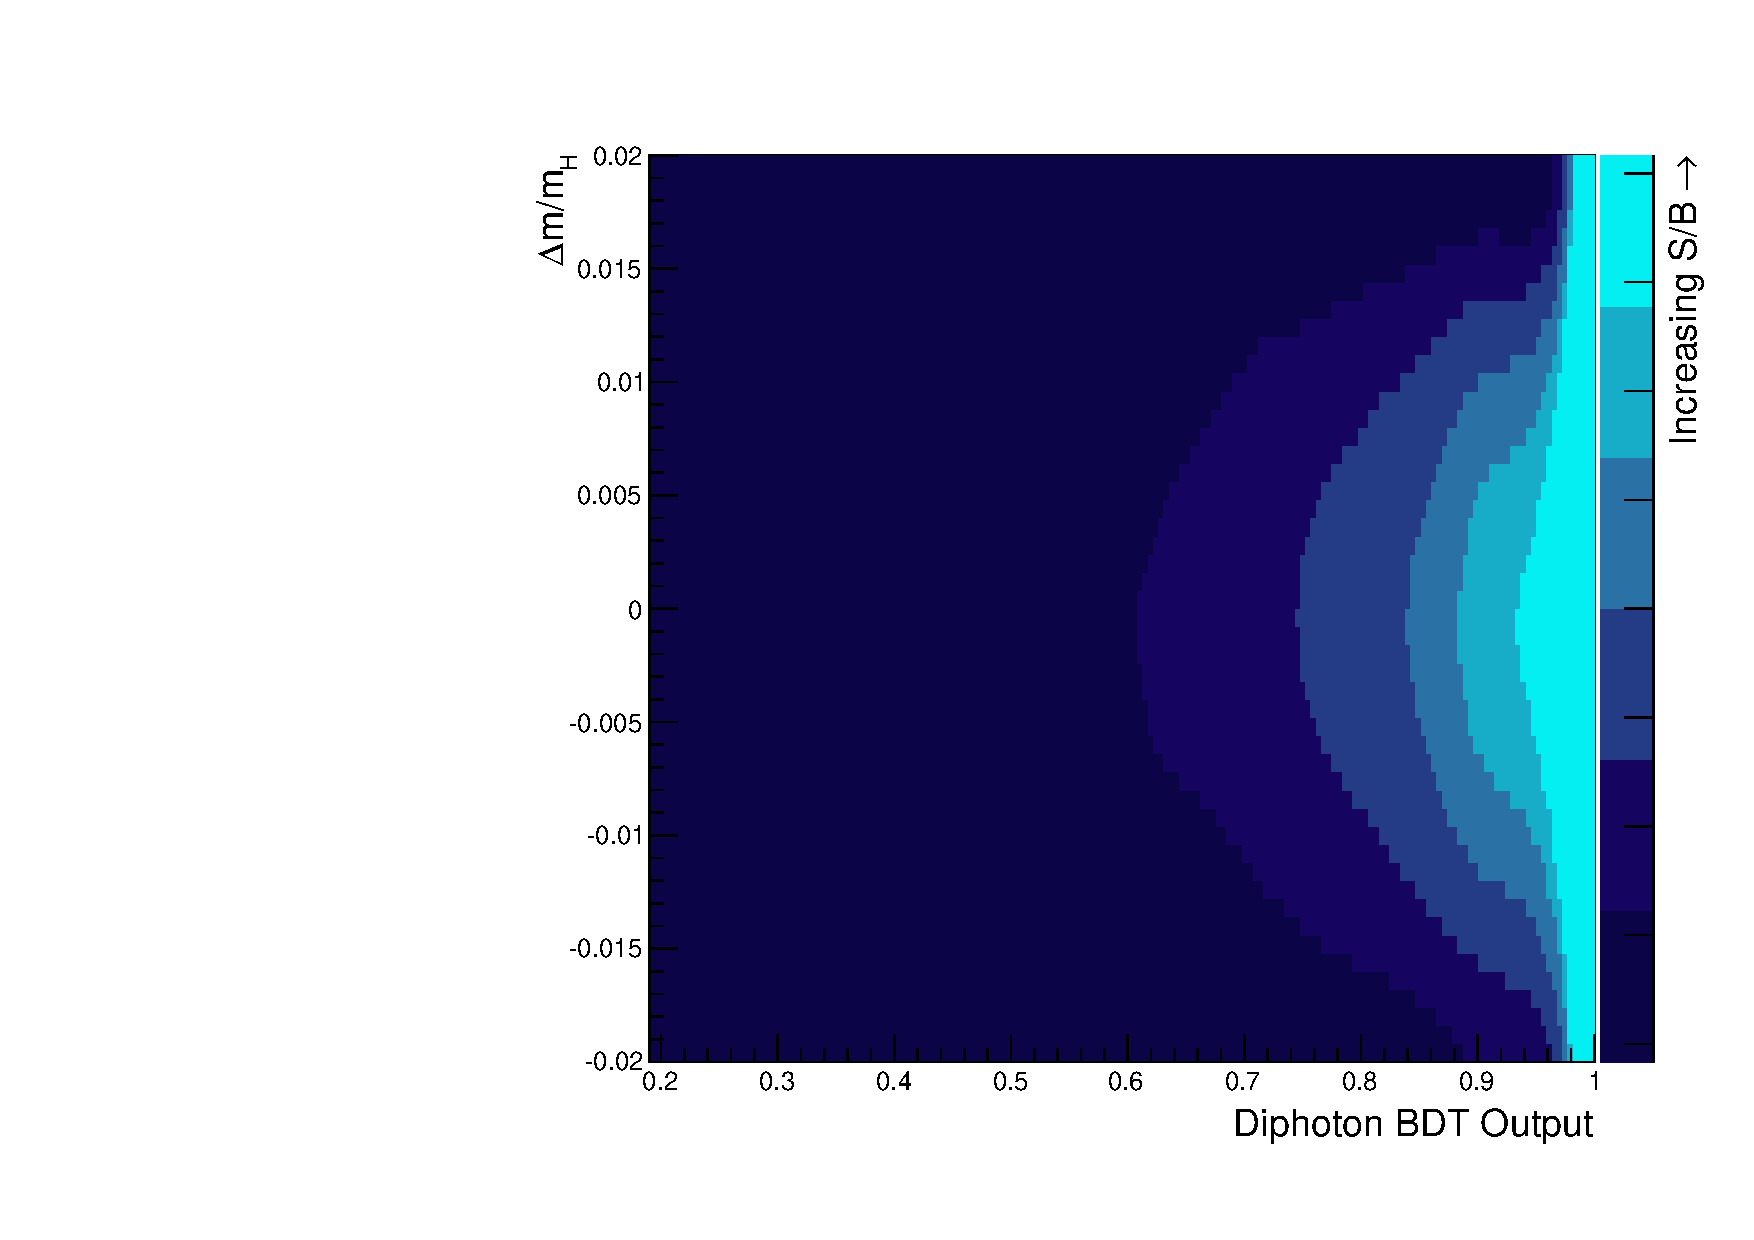
\includegraphics[width=0.48\textwidth]{selec_and_cats/plots/sideband_cats_7TeV.pdf}
  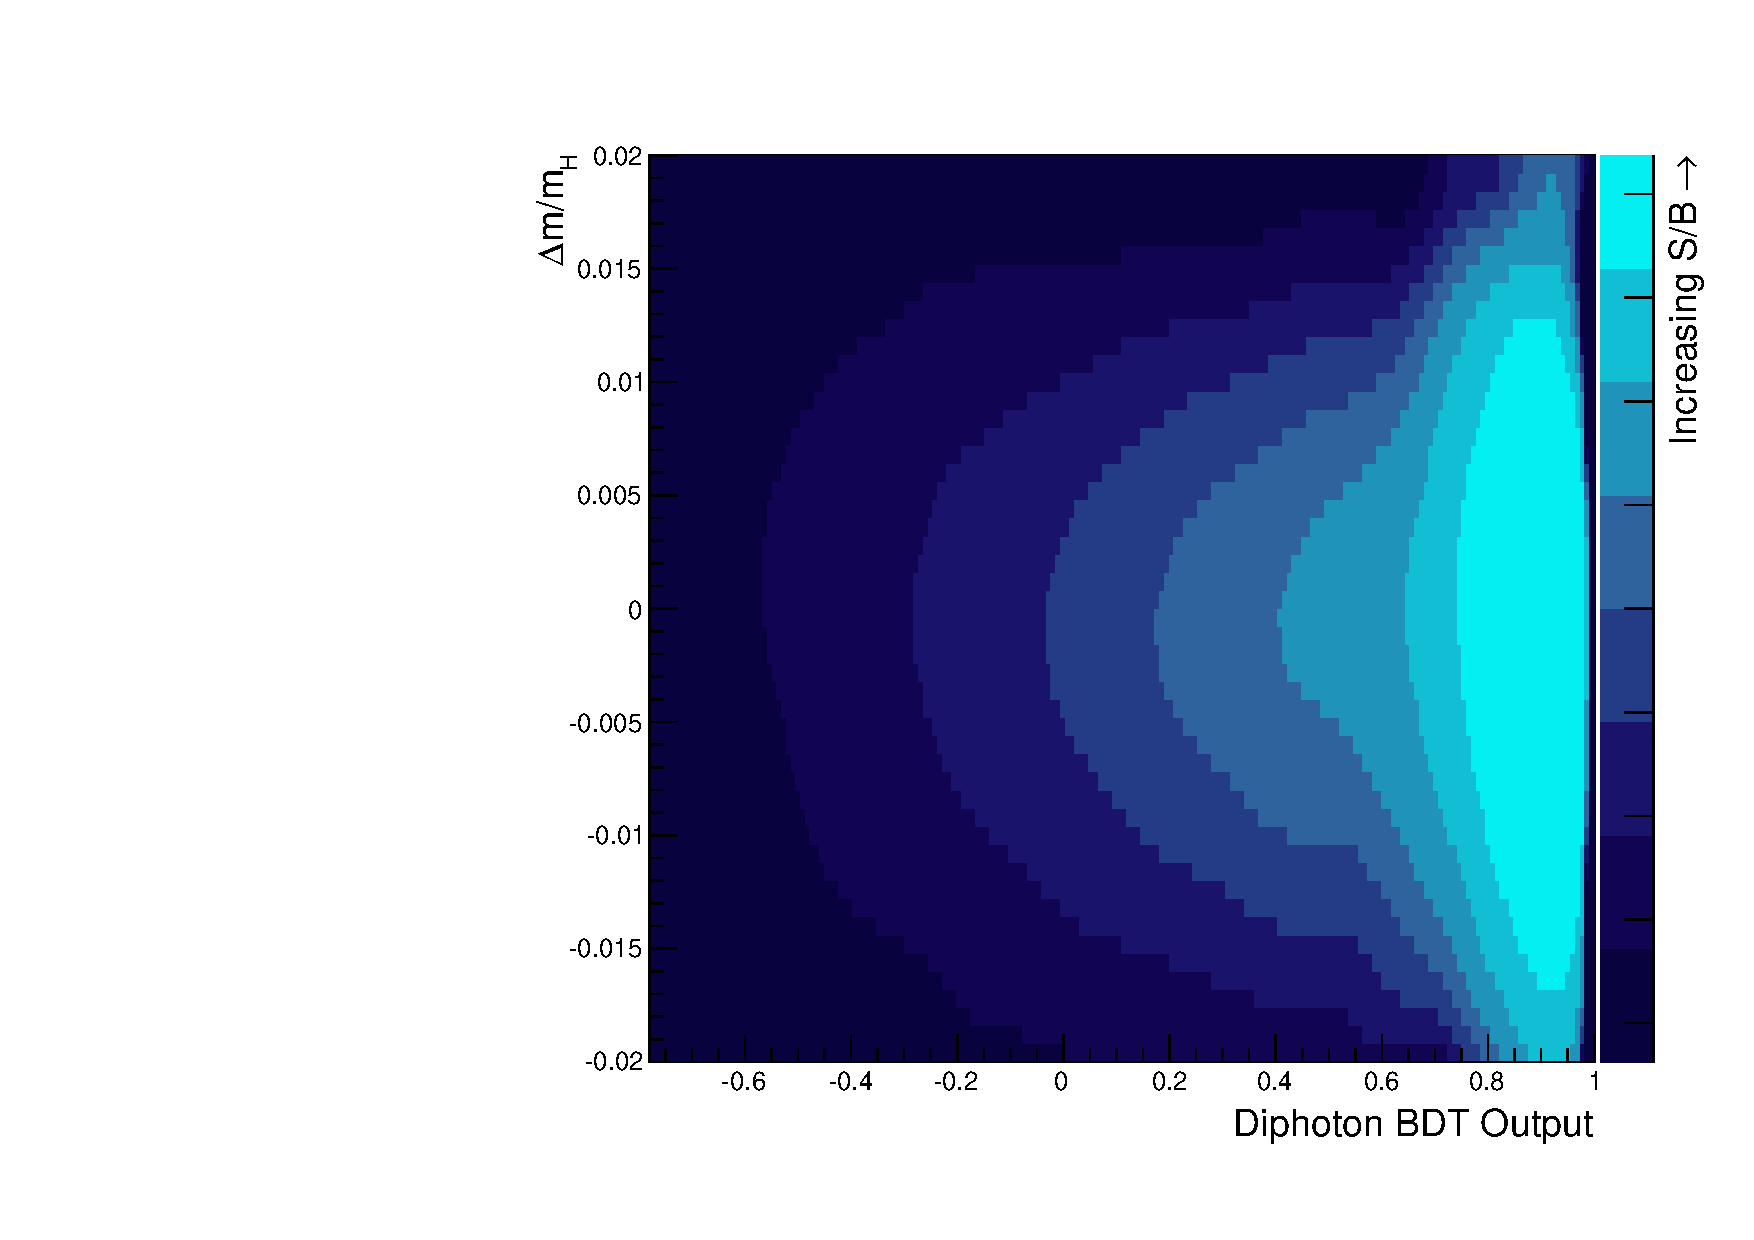
\includegraphics[width=0.48\textwidth]{selec_and_cats/plots/sideband_cats_8TeV.pdf}
  \caption{The inclusive category bin definitions for the \SMVA analysis. Shown for the 7~\TeV dataset on the left and the 8~\TeV dataset on the right.}
  \label{fig:sideband_cats}
\end{figure}

\subsection{Event categorisation summary}

All the categories and the tagging order are summarised in the table below (Table~\ref{tab:cat_summary}).

\begin{table}[h!]
\caption{The event classes at 7 and 8\TeV and some of their main selection requirements. Events are tested against the selection requirements
of the classes in the order they are listed here.}
\begin{center}
\begin{tabular}{l c c p{10cm}}
\multirow{2}{*}{Label} & \multicolumn{2}{l}{No. of classes} & \multirow{2}{*}{Main requirements} \\
 & 7\GeV & 8\GeV & \\
\hline
\multirow{3}{*}{\ttH lepton tag} & \multirow{3}{*}{$\star$} & \multirow{3}{*}{1} & $\ptga>\mgg/2$ \\ %% $\text{diphoton BDT}>-0.6$
                                                                               & & & 1 b-tagged jet + 1 electron or muon \\
                                                                               & & & \textbf{For MVAs:} diphoton BDT $>0.6(-0.6)$ at 7(8)~\TeV \\
\hline
\multirow{4}{*}{\VH tight $\ell$ tag} & \multirow{4}{*}{1} & \multirow{4}{*}{1} & $\ptga>45\cdot\mgg/120$ \\ %% $\text{diphoton BDT}>-0.6$
                                                                  & & & $e$ or $\mu$, $\pT>20\GeV$, and $\MET>45\GeV$ OR\\
                                                                  & & & $2e$ or $2\mu$, $\pT>10\GeV$; $70<m_{ll}<110\GeV$ \\
                                                                  & & & \textbf{For MVAs:} diphoton BDT $>0.1(-0.6)$ at 7(8)~\TeV \\
\hline
\multirow{3}{*}{\VH loose $\ell$ tag} & \multirow{3}{*}{1} & \multirow{3}{*}{1} & $\ptga>45\cdot\mgg/120$ \\ %%  $\text{diphoton BDT}>-0.6$
                                                                   & & & $e$ or $\mu$, $\pT>20\GeV$ \\
                                                                   & & & \textbf{For MVAs:} diphoton BDT $>0.1(-0.6)$ at 7(8)~\TeV \\

\hline
\multirow{3}{*}{\VBF dijet tag} & \multirow{3}{*}{2} & \multirow{3}{*}{2/3$^{\dagger}$} & $\ptga>\mgg/2$ \\
                                                                             & & & \textbf{For MVAs:} 2 jets; dijet and combined diphoton-dijet BDTs used\\
                                                                             & & & \textbf{For CiC:} 2 jets, cut based dijet selection used \\
\hline
\multirow{3}{*}{\VH \MET\ tag} & \multirow{3}{*}{1} & \multirow{3}{*}{1} & $\ptga>45\cdot\mgg/120$\\ %% , $\text{diphoton BDT}>0.0$ 
                                                                    & & & $\MET>70\GeV$ \\
                                                                    & & & \textbf{For MVAs:} diphoton BDT $>0.8(0.0)$ at 7(8)~\TeV \\ 

\hline
\multirow{3}{*}{\ttH multijet tag} & \multirow{3}{*}{$\star$} & \multirow{3}{*}{1} & $\ptga>\mgg/2$ \\ %% , $\text{diphoton BDT}>-0.3$
                                                                       & & & 1 b-tagged jet + 4 more jets \\
                                                                       & & & \textbf{For MVAs:} diphoton BDT $>0.6(-0.2)$ at 7(8)~\TeV \\ 
\hline
\multirow{3}{*}{\VH dijet tag} & \multirow{3}{*}{1} & \multirow{3}{*}{1} & $\ptga>45\cdot\mgg/120$\\ %% , $\text{diphoton BDT}>0.2$ 
                                                                                         & & & jet pair, $\pT>40\GeV$ and $60<\mjj<120\GeV$ \\
                                                                                         & & & \textbf{For MVAs:} diphoton BDT $>0.6(0.2)$ at 7(8)~\TeV \\ 

\hline
\multirow{3}{*}{Untagged} & \multirow{3}{*}{4/8$^{\ddagger}$} & \multirow{3}{*}{5/8/10$^{\ddagger}$} & The remaining events,\\
                                                                          & &  & \textbf{For MVAs:} classified using diphoton BDT \\
                                                                          & & & \textbf{For CiC:} classified using \eta and \rnine of photons and $p_{T}^{\gamma\gamma}/m_{\gamma\gamma}$ \\
\hline
\multicolumn{4}{ p{16cm} }{$\star$ For the 7\TeV dataset, events in the \ttH lepton tag and multijet tag classes are combined,
after selection, to form a single event class.} \\
\multicolumn{4}{ p{16cm} }{$\dagger$ For the CiC (MVA) analysis there are 2 (3) dijet categories at 8~\TeV.} \\
\multicolumn{4}{ p{16cm} }{$\ddagger$ For the CiC analysis there are 8 inclusive categories at 7 and 8~\TeV, for the MFM there are 4 (5) categories at 7 (8)~\TeV and for the SMVA there are 8 (10).} \\
\end{tabular}
\end{center} 
\label{tab:cat_summary}
\end{table}

%\begin{table}[h!]
%  \begin{center}
%    \begin{tabular}{l | l l l l l l}
%      \multirow{3}{*}{Category type} & \multicolumn{6}{c}{Number of categories} \\
%      & \multicolumn{2}{c}{\CiC} & \multicolumn{2}{c}{\MFM} & \multicolumn{2}{c}{\SMVA} \\
%      & 7~\TeV & 8~\TeV & 7~\TeV & 8~\TeV & 7~\TeV & 8~\TeV \\
%      \hline
%      Inclusive & 8 & 8 & 4 & 5 & 8 & 10 \\
%      \VBF tagged & 2 & 2 & 2 & 3 & 2 & 3 \\
%      \VH tagged & 4 & 4 & 4 & 4 & 4 & 4 \\
%      \ttH tagged & 1 & 2 & 1 & 2 & 1 & 2 \\
%    \end{tabular}
%    \caption{A summary of the number of categories for each of the analyses.}
%    \label{tab:cat_summary}
%  \end{center}
%\end{table}
